\documentclass{beamer}
\usetheme{Madrid}

\usepackage[utf8]{inputenc}
\usepackage{graphicx}
\usepackage{booktabs}
\usepackage{hyperref}
\usepackage{color}
\usepackage{natbib}
\usepackage{aastex-compat}
\usepackage{siunitx}
\usepackage{aas_macros}
\usepackage{amsmath}
\title[PhD Thesis]{Estudio de la Interacción de Flujos Múltiples de Fuentes Astrofísicas, Aplicada a los Proplyds Clásicos de la Nebulosa de Orión}
\author[M.C Jorge Alejandro Tarango Yong]{Presents: M.C Jorge Alejandro Tarango Yong \\
  PhD Advisor: Dr. William Henney \\
  Tutorial Committee: Dr. Javier Ballesteros, Dr. Luis Zapata}
\date{\today}
\definecolor{AZUL}{HTML}{000032}
\definecolor{DORADO}{HTML}{A87A00}
\setbeamercolor{title}{fg=AZUL, bg=DORADO}
\setbeamercolor{frametitle}{fg=AZUL, bg=DORADO}
\setbeamercolor{structure}{fg=AZUL, bg=DORADO}
\setbeamertemplate{enumerate items}[square]
\setbeamertemplate{section in toc}[square]
\newcommand\thC{\(\theta^1\)\,Ori~C}
\newcommand\Ion[2]{\ensuremath{\mathrm{#1\,\scriptstyle #2}}} %Used when naming different ions. Credit: William J. Henney
\newcommand{\twocols}[2]{
  \begin{columns}
    \begin{column}{5.8cm}
      #1
    \end{column}
    \begin{column}{5.8cm}
      #2
    \end{column}
  \end{columns} 
}

\newcommand{\twocolspic}[2]{
  \begin{columns}
    \begin{column}{4.2cm}
      #1
    \end{column}
    \begin{column}{7.6cm}
      #2
    \end{column}
  \end{columns} 
}

\AtBeginSection[]{%
\begin{frame}
    \tableofcontents[currentsection, subsectionstyle=show/show/hide]
\end{frame}
}

\begin{document}
\frame{\frametitle{PhD Thesis Defense}
  
\includegraphics[scale=0.1]{../Figures/logo}
  \maketitle}

\frame{\frametitle{Index}
  \tableofcontents}
\section{Introduction}
\frame{\frametitle{Motivation of this work}
  \twocols{\begin{block}{}
      Bow shocks occur in many kinds of astrophysical scenarios, from galactic to planetary scales. In this work we develop a mathematical tool for characterizing cylindrically symmetric, geometrically thin and optically thin bow shocks based into their geometrical shape and how is oriented respect the plane of sky.
    \end{block}}{\begin{block}{}
      \begin{center}
        \includegraphics[width=0.6\linewidth]{../Figures/collage}
      \end{center}
    \end{block}}
}

\frame{
  \begin{block}{We called it the $\Lambda'-\Pi'$ diagram \citep{Tarango-Yong:2018a}.}
    \begin{center}
      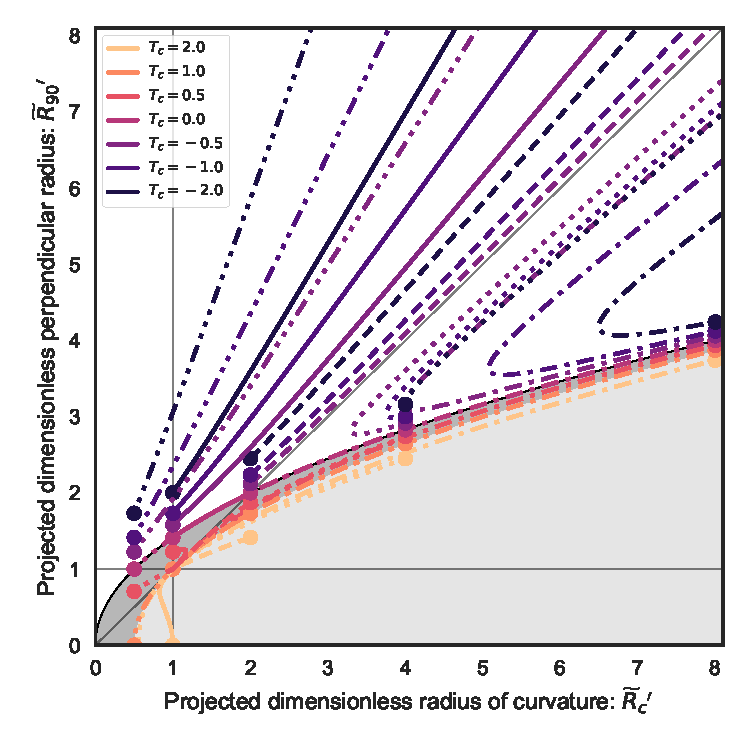
\includegraphics[width=0.6\linewidth]{../Figures/projected-R90-vs-Rc}
    \end{center}
    
    \end{block}
 }
\frame{
  \twocols{\begin{block}{}{
Then we apply this tool to the simplest mathematical surfaces: the quadrics of revolution \citep{Goldman:1983a, Gfrerrer:2009a} and to a simple model for winds interaction: the Thin Shell Model \citep{Canto:1996}.
      }\end{block}}{\begin{block}{}{
        \includegraphics<1>[width=\linewidth]{../Figures/collage2}
        \includegraphics<2>[width=\linewidth]{../Figures/ancantoid-R90-vs-Rc-a}
      }\end{block}}
}
\frame{
  \twocols{\begin{block}{}
      And finally compare the thin shell model against observations of the classical proplyds of the Trapezium in the core of the Orion Nebula in a similar diagram.
    \end{block}}{\begin{block}{}
      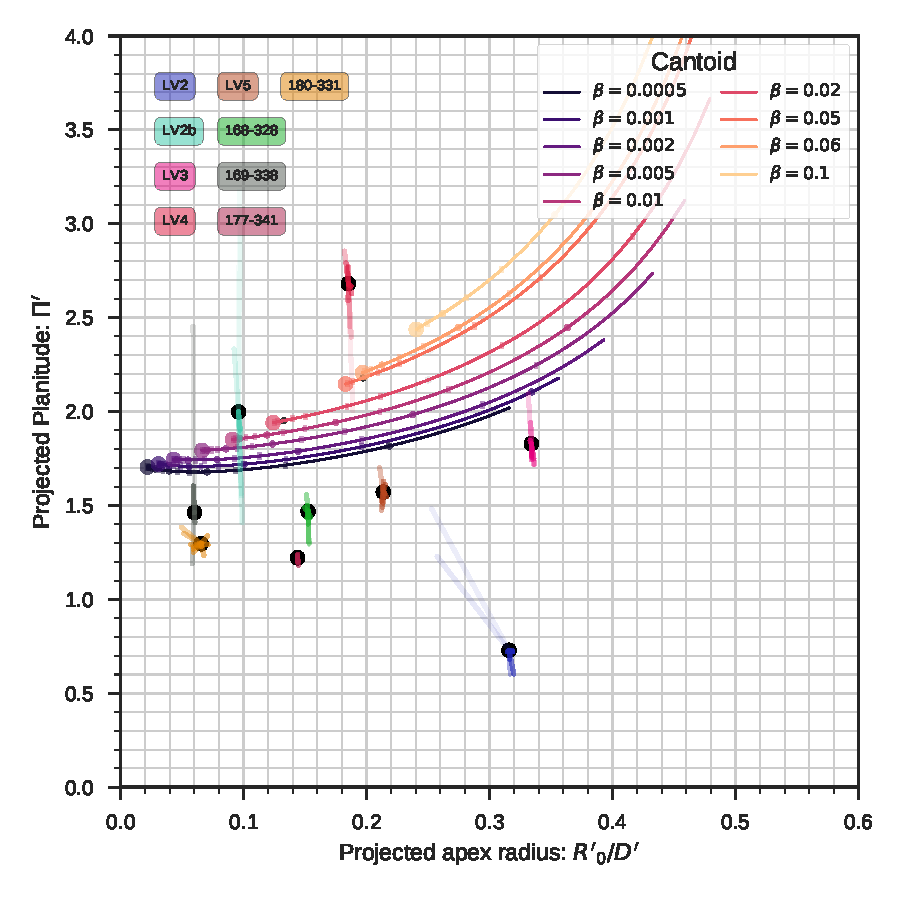
\includegraphics[width=\linewidth]{../Figures/obs-diagnostic-Pi-R0-Cantoid}
    \end{block}}
}
\section{Bow Shocks in the ISM}
\frame{\frametitle{Bow Shocks in the ISM}
  \twocols{\begin{block}{}
      Bow shocks are emmision arcs produced when some fluid interacts at supersonic speeds with another object. Some astrophysical examples seen in the Interstellar Medium (ISM) are:
      \begin{itemize}
      \item \textbf{Jets Surface Work}
      \item Magnetosphere interaction with stellar wind
      \item Stellar Bow shocks
        \begin{itemize}
        \item AGB stars and red supergiants
        \item Runaway O stars
        \item Proplyds
        \item T Tauri stars
        \item Neutron stars
        \end{itemize}
      \end{itemize}
    \end{block}}{\begin{block}{}
      \includegraphics[width=\linewidth]{../Figures/CygnusA} \\
      \footnotesize Cygnus A \citep{Perley:1984}\end{block}
    }
  }

\frame{\frametitle{Bow Shocks in the ISM}
  \twocols{\begin{block}{}
      Bow shocks are emmision arcs produced when some fluid interacts at supersonic speeds with another object. Some astrophysical examples seen in the Interstellar Medium (ISM) are:
      \begin{itemize}
      \item Jets Surface Work
      \item \textbf{Magnetosphere interaction with stellar wind}
      \item Stellar Bow shocks
        \begin{itemize}
        \item AGB stars and red supergiants
        \item Runaway O stars
        \item Proplyds
        \item T Tauri stars
        \item Neutron stars
        \end{itemize}
      \end{itemize}
    \end{block}}{\begin{block}{}
      \includegraphics[width=\linewidth]{../Figures/HJ-Yates}\\
      \footnotesize Density of material flowing from a Hot Jupiter through magnetosphere interacting with stellar wind \citep{Yates:2018}.\end{block}
    }
  }

\frame{\frametitle{Bow Shocks in the ISM}
  \twocols{\begin{block}{}
      Bow shocks are emmision arcs produced when some fluid interacts at supersonic speeds with another object. Some astrophysical examples seen in the Interstellar Medium (ISM) are:
      \begin{itemize}
      \item Jets Surface Work
      \item Magnetosphere interaction with stellar wind
      \item Stellar Bow shocks
        \begin{itemize}
        \item \textbf{AGB stars and red supergiants}
        \item Runaway O stars
        \item Proplyds
        \item T Tauri stars
        \item Neutron stars
        \end{itemize}
      \end{itemize}
    \end{block}}{\begin{block}{}
      \includegraphics[width=\linewidth]{../Figures/cox-betelgeuse}\\
      \footnotesize Observation of a ``Fermata'' type bow shock at \SI{70}{\mu.m} produced by the interaction of the strong wind of a red supergiant ($\alpha$\,Ori) with the ISM \citep{Cox:2012}.\end{block}
    }
  }

\frame{\frametitle{Bow Shocks in the ISM}
  \twocols{\begin{block}{}
      Bow shocks are emmision arcs produced when some fluid interacts at supersonic speeds with another object. Some astrophysical examples seen in the Interstellar Medium (ISM) are:
      \begin{itemize}
      \item Jets Surface Work
      \item Magnetosphere interaction with stellar wind
      \item Stellar Bow shocks
        \begin{itemize}
        \item AGB stars and red supergiants
        \item \textbf{Runaway O stars}
        \item Proplyds
        \item T Tauri stars
        \item Neutron stars
        \end{itemize}
      \end{itemize}
    \end{block}}{\begin{block}{}
      \begin{center} 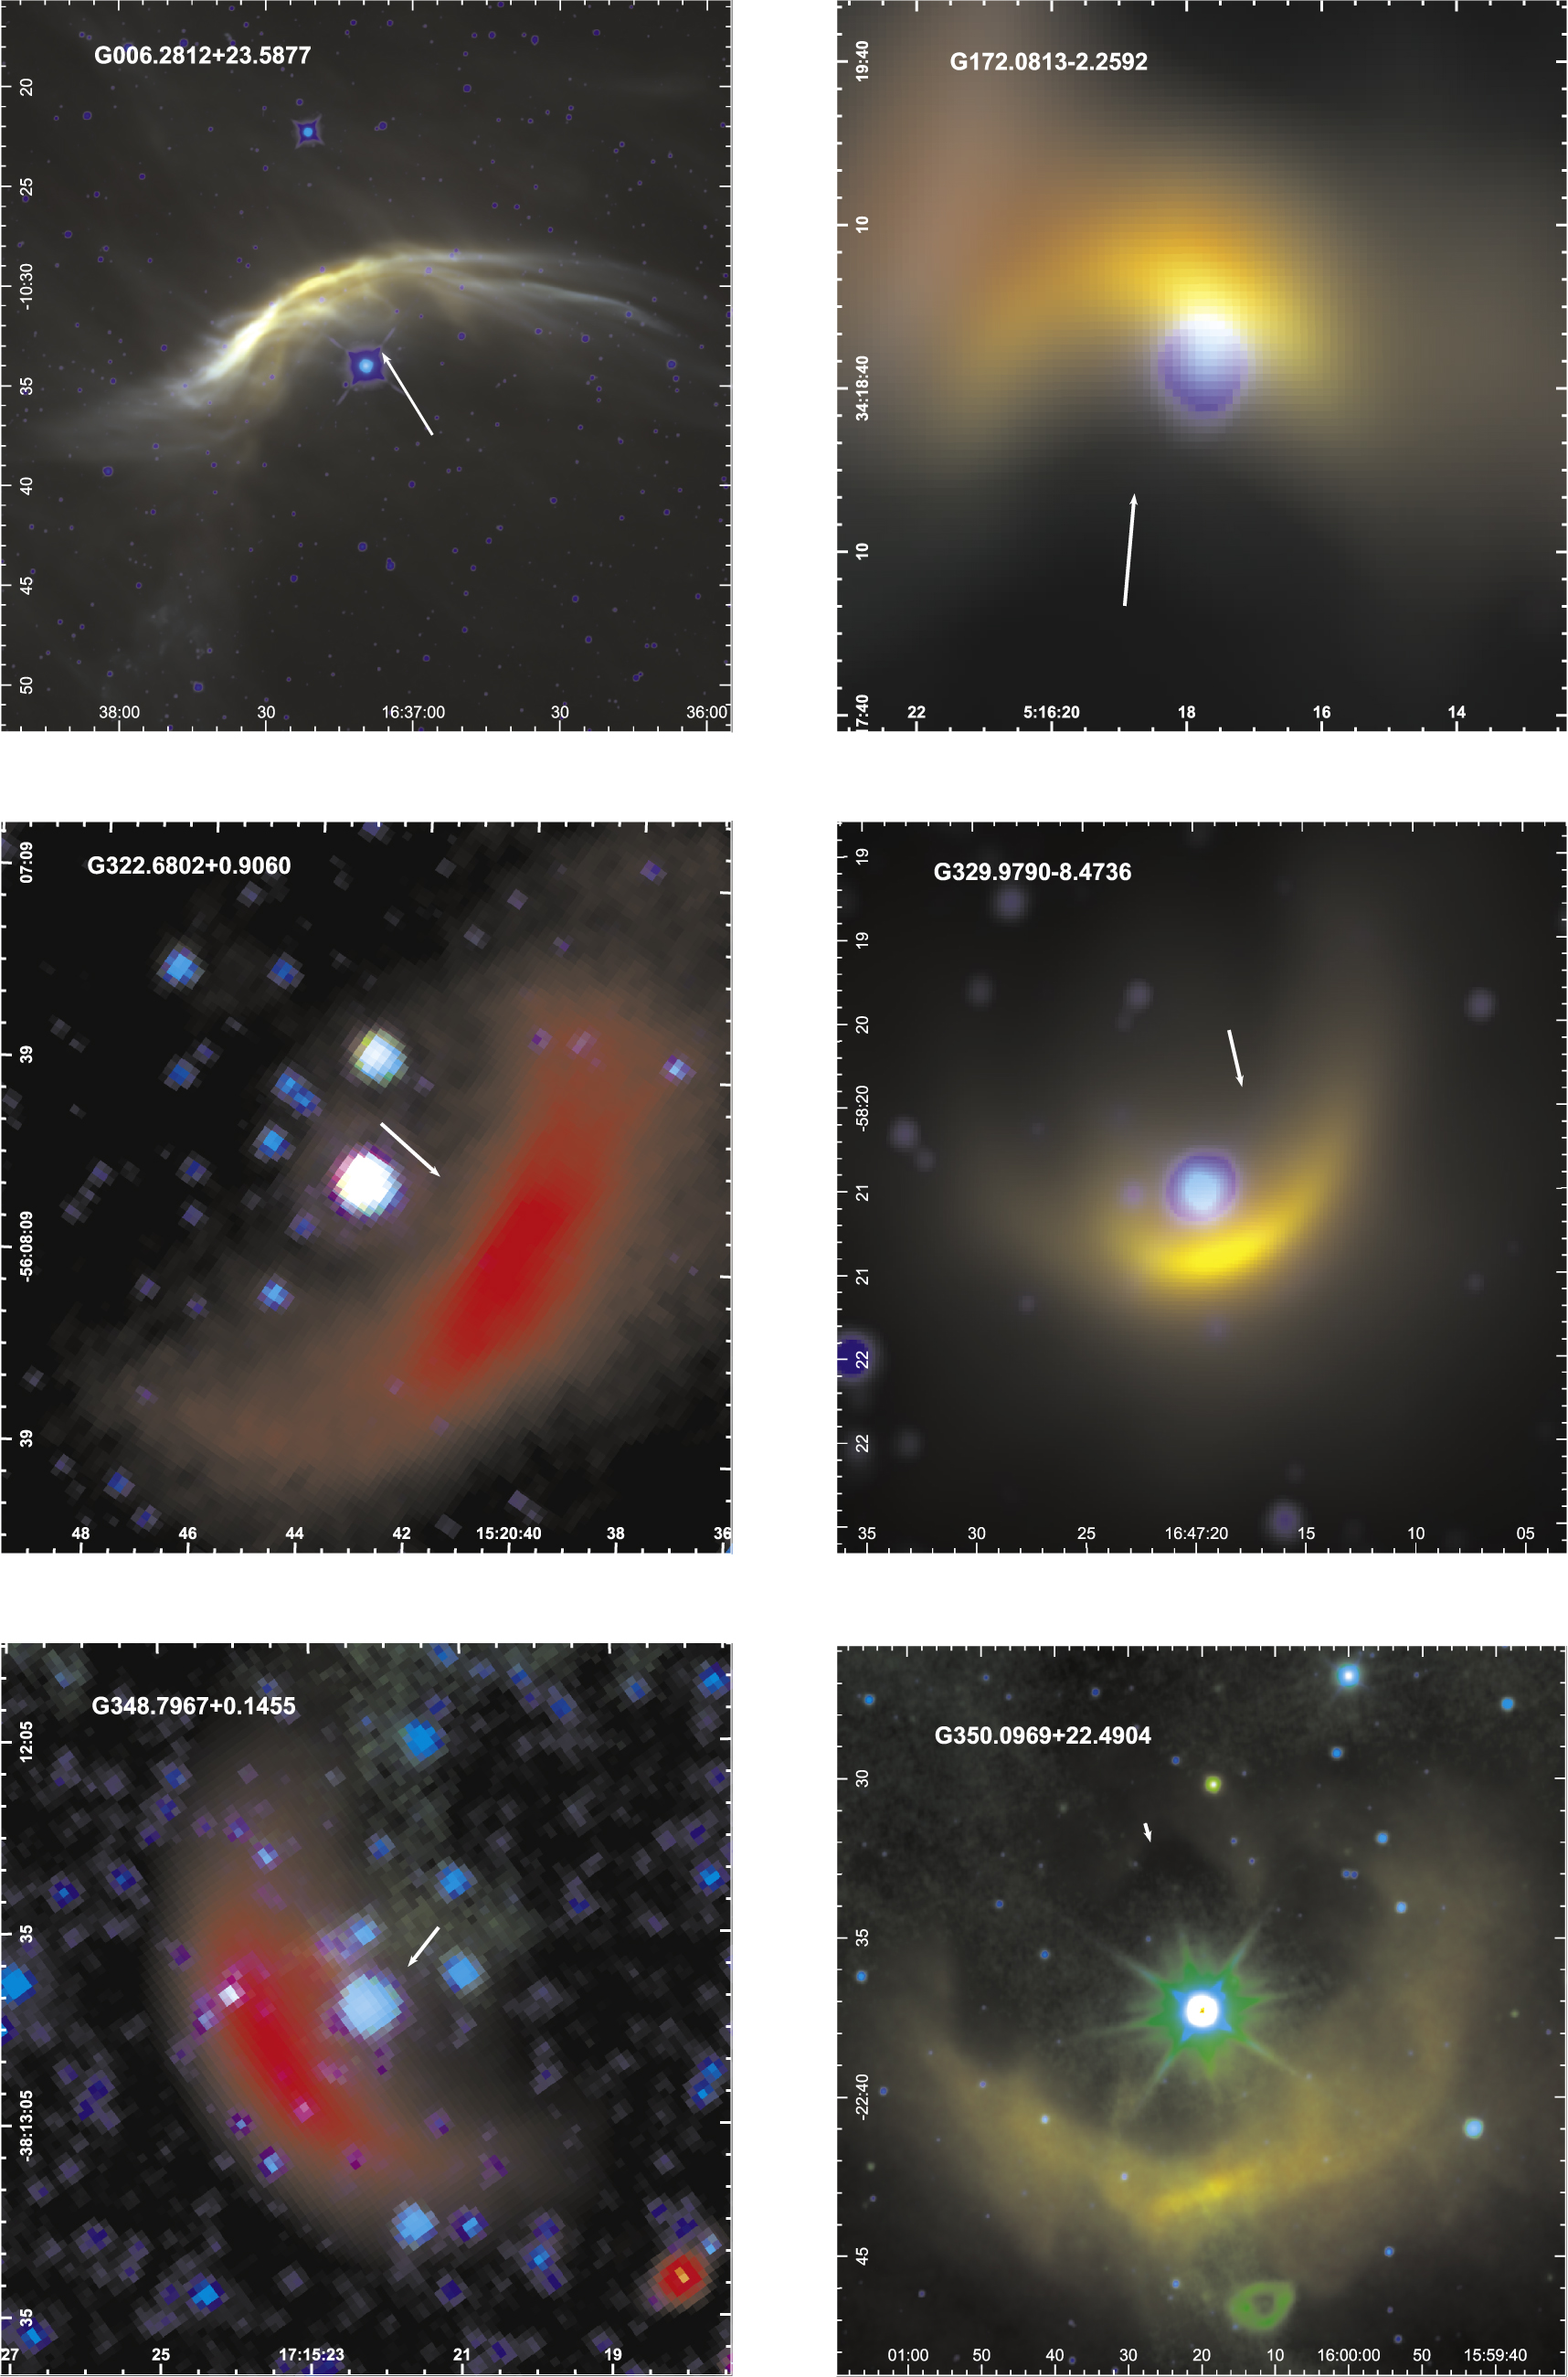
\includegraphics[width=0.5\linewidth]{../Figures/kobulnicky}\end{center}\\
       \footnotesize Observations of prototypical examples of ``Bow shock nebulae'' by Spitzer or WISE produced by runaway stars interacting with the ISM (red: 20 or \SI{22}{\mu.m}, green:8 or \SI{12}{\mu.m}, blue: \SI{4.5}{\mu.m})\citep{Kobulnicky:2016}.\end{block}
    }
  }
  
\frame[label=bally]{\frametitle{Bow Shocks in the ISM}
  \twocols{\begin{block}{}
      \small
      Bow shocks are emmision arcs produced when some fluid interacts at supersonic speeds with another object. Some astrophysical examples seen in the Interstellar Medium (ISM) are:
      \begin{itemize}
      \item Jets Surface Work
      \item Magnetosphere interaction with stellar wind
      \item Stellar Bow shocks
        \begin{itemize}
        \item AGB stars and red supergiants
        \item Runaway O stars
        \item \textbf{Proplyds}
        \item T Tauri stars
        \item Neutron stars
        \end{itemize}
      \end{itemize}
    \end{block}}{\begin{block}{}
      \begin{center}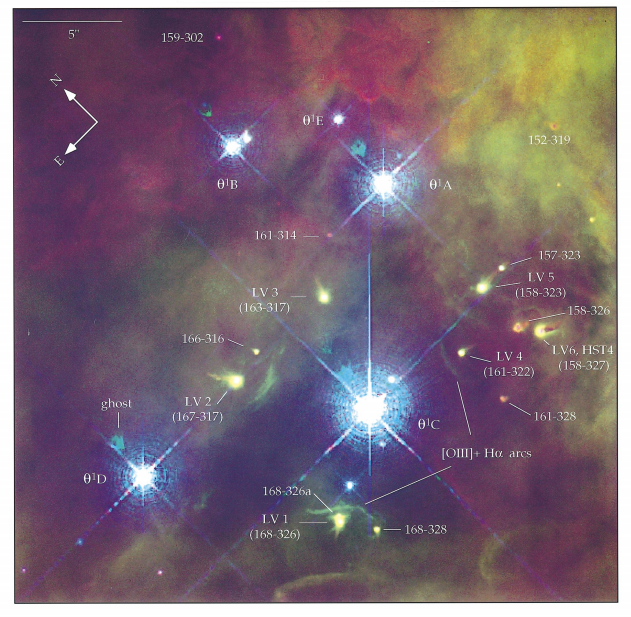
\includegraphics[width=0.8\linewidth]{../Figures/bally-trapezium}\end{center}\\
      \footnotesize  The Classical proplyds in the core of the trapezium in Orion Nebula also show a bow shock by the HST (red is [\Ion{N}{II}], green is \Ion{H}{\alpha} and blue is [\Ion{O}{I}]) \citep{Bally:1998}.\end{block}}
  \tiny \hyperlink{Robberto}{\beamergotobutton{Return button}}
}
\section{Orion Nebula}
\frame{\frametitle{Orion Nebula}
  \twocolspic{\begin{block}{}
      The Orion Nebula is the nearest \Ion{H}{II} region ($\sim \SI{414}{pc}$, \citet{Menten:2007}), where massive star formation can be studied with high resolution observations.
    \end{block}}{\begin{block}{}
      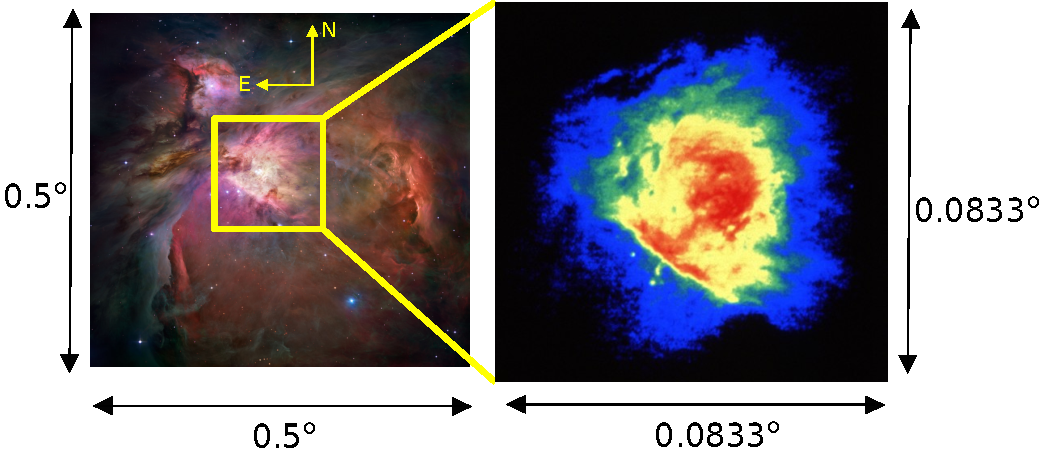
\includegraphics[width=\linewidth]{../Figures/orion-HST-NRAO} \\
      www.hubblesite.org
    \end{block}}
}
\frame{\frametitle{Proplyds in Orion Nebula}
  \twocols{\begin{block}{}About 70 arcs have been detected within Orion Nebula \citep{Gutierrez-Soto:2015a}, many of them are produced by proplyds.\end{block}}{\begin{block}{}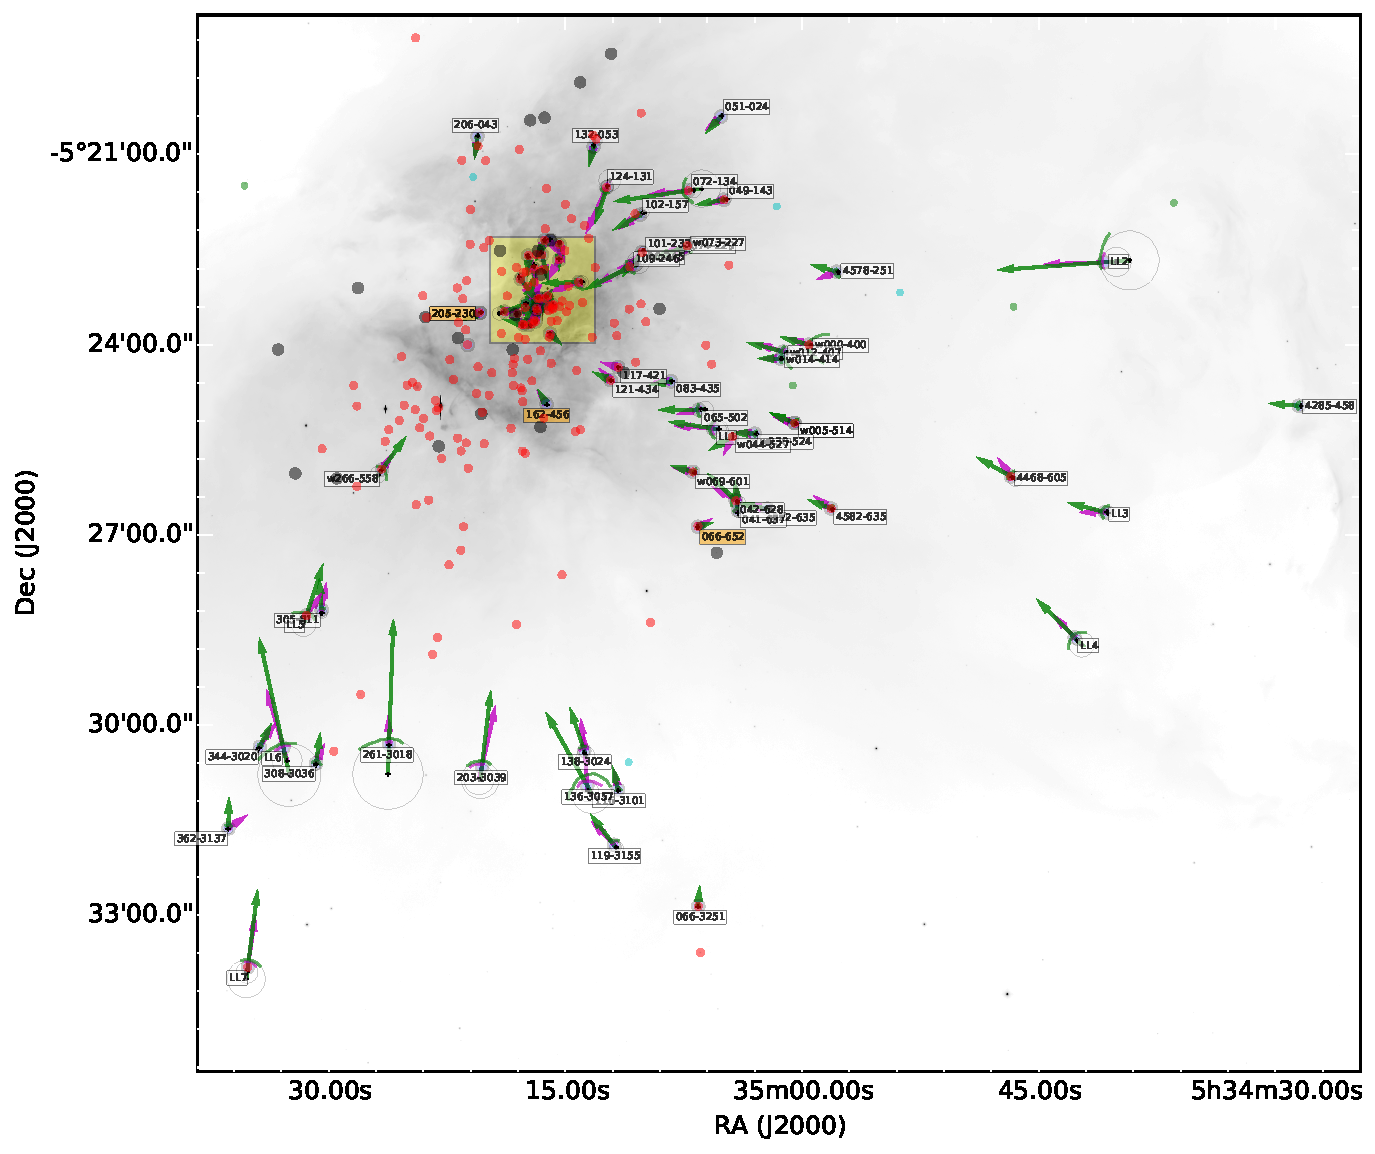
\includegraphics[width=\linewidth]{../Figures/ll-pos-image-Luis} \\
    \footnotesize  Map of bow shocks in Orion Nebula \citep{Gutierrez-Soto:2015a}
    \end{block}}
}

\frame{\frametitle{Proplyds in Orion Nebula}
  \twocols{\begin{block}{}About 70 arcs have been detected within Orion Nebula \citep{Gutierrez-Soto:2015a}, many of them are produced by proplyds.\end{block}}{\begin{block}{}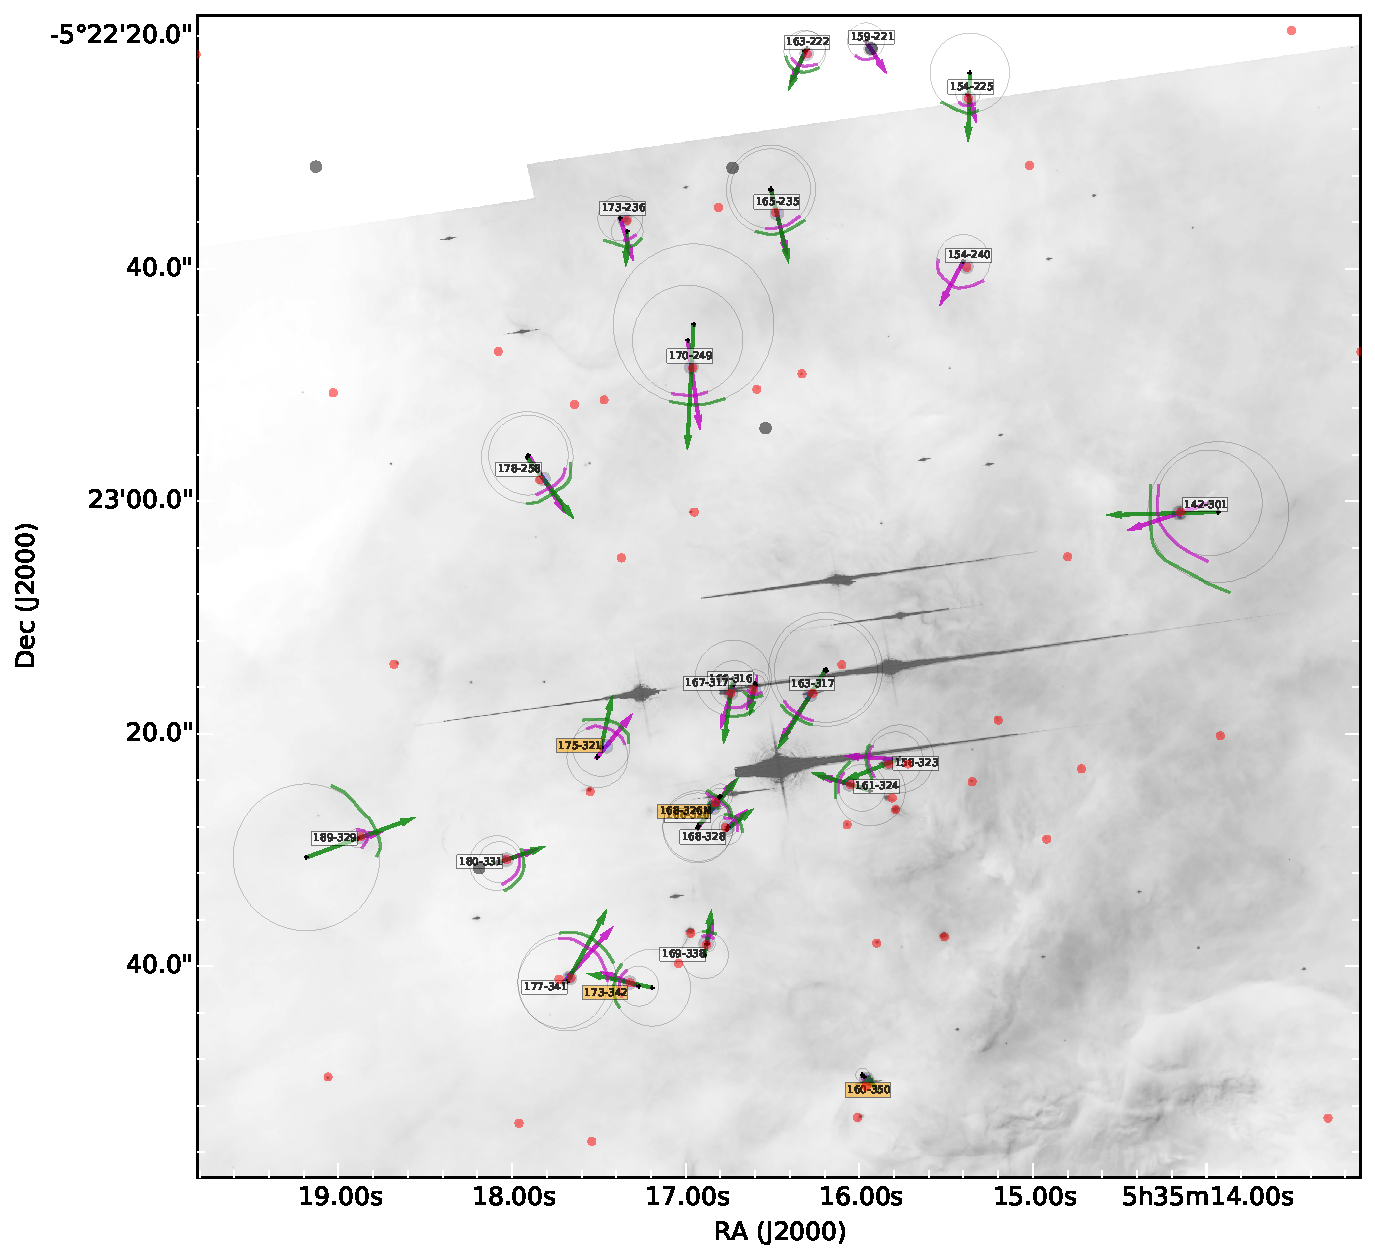
\includegraphics[width=\linewidth]{../Figures/ll-pos-image-zoom-Luis} \\
    \footnotesize  Map of bow shocks in Orion Nebula (Trapezium zoomed) \citep{Gutierrez-Soto:2015a}
    \end{block}}
}

\frame[label=Robberto]{
  \twocols{\begin{block}{}
      Some of the nearest proplyds to \thC{} were previously observed by \citet{Bally:1998} \hyperlink{Rob-image}{\beamergotobutton{Go to image}} and \citet{Robberto:2005} in mid infrared and their shape analyzed using the Thin Shell Model from \citep{Canto:1996}, but some proplyds don't fit at all.
    \end{block}}{\begin{block}{}
      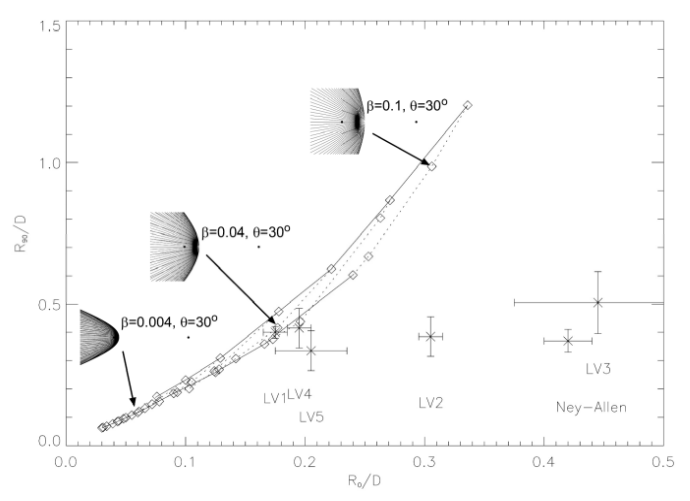
\includegraphics[width=\linewidth]{../Figures/robberto} \\
      \footnotesize Apparent shape of some proplyds (in black points) compared with the thin shell model of \citep{Canto:1996} (open dots and lines) in a $R_{90}/D$ vs $R_0/D$ diagram \citep{Robberto:2005}.
    \end{block}}
}
\frame[label=k-index]{
  
  \begin{block}{}
    \begin{center}
      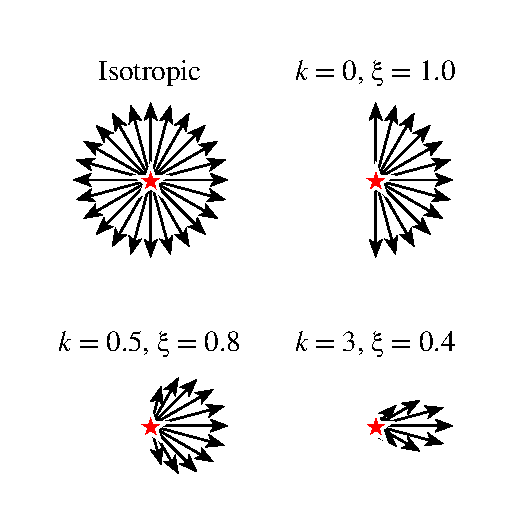
\includegraphics[width=0.5\linewidth]{../Figures/anisotropic-arrows}
      \end{center} \\
      \footnotesize This motivated us to extend \citet{Canto:1996} model to include non isotropic winds.

      \hyperlink{generic-bow}{\beamergotobutton{Return Button}}
    \end{block}
}
\frame{\frametitle{Photoevaporated wind in proplyds}
  \twocols{\begin{block}{}
      Proplyds are bright structures with cometary shape which are the result of the photoevaporation of a protoplanetary disk (hence the name) due to a strong source of ultraviolet radiation (e.g a massive star).
    \end{block}}{\begin{block}{}
      \begin{center}
        \includegraphics[width=0.6\linewidth]{../Figures/HST10}
        \end{center} \\
      \footnotesize HST10 is the archetypical example of a proplyd. Image taken with the HST (red: F656N filter, green: F658N, blue: F631N filter, \citet{Tsamis:2013}).
    \end{block}}
}

\frame{
  \twocols{\begin{block}{}
      The incident UV radiation photoevaporates the gas in the protoplanetary disk, which becomes a spherical flow due to pressure gradients. Only the gas located at $r > r_g = \frac{GM_*}{a^2}$ (where $M_*$ is the mass of the central star and $a$ is the speed of sound of the gas) can escape from the disk.
      \end{block}}{\begin{block}{}
      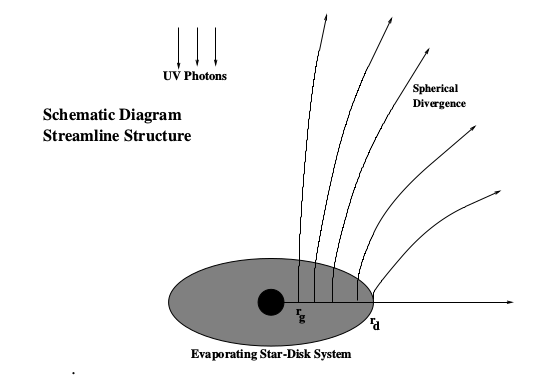
\includegraphics[width=\linewidth]{../Figures/Johnstone-1}
    \end{block}}
}
\frame{
  \twocolspic{\begin{block}{}
      The head is shaped by the incident UV radiation from the massive star, forming a D type Ionization Front, while the tail is shaped by diffuse and ionizing radiation.
    \end{block}
}{ \begin{block}{}
    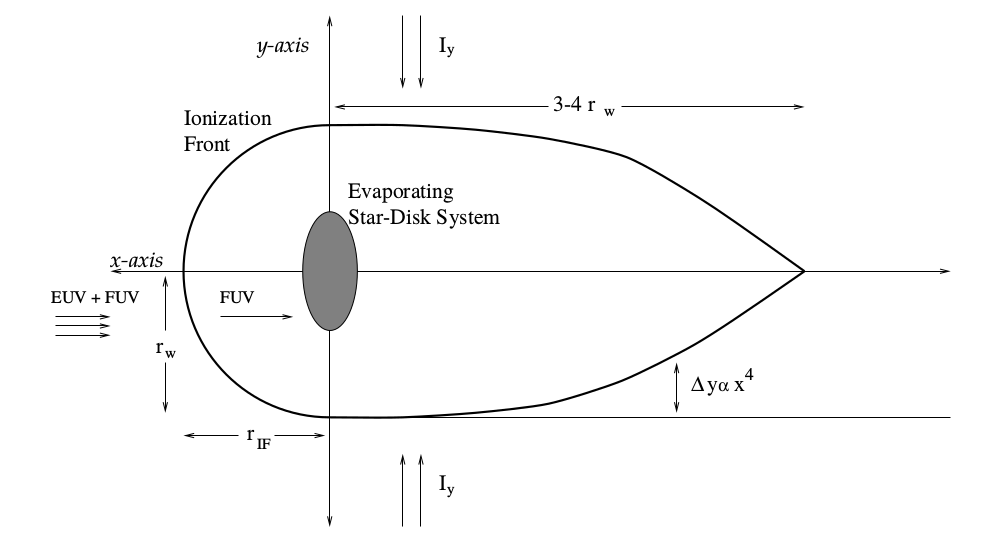
\includegraphics[width=\linewidth]{../Figures/Johnstone-shape} \\
    \citep{Johnstone:1998}
  \end{block}
  
}
}
%\frame{}
\section{Fundamental Concepts}
\frame[label=generic-bow]{\frametitle{General Considerations}
  \begin{block}{}
    For our model for the two winds interaction which forms a bow shock we consider two main scenarios:
  \end{block}
  \twocols{\begin{block}{}
      \only<1>{Two wind sources separated by a distance $D$ from each other. The weaker wind is placed at the origin and has any of the profiles of \hyperlink{k-index}{\beamergotobutton{slide 16}}, while the stronger wind is spherical and isotropic.}
      \includegraphics<2>[width=\linewidth]{../Figures/wilkinoid}
      \end{block}
    }{\begin{block}{}
        \includegraphics<1>[width=\linewidth]{../Figures/bowshock-crw-variables}
        \only<2>{The second scenario is a spherical, isotropic wind placed at the origin interacting with a plane-parallel flow with constant density}
      \end{block}
  }
}

\frame{\frametitle{General Considerations}
  \begin{block}{}
    \twocols{The shape of the bow shock is determined by the function $R(\theta, \phi)$, where $(\theta, \phi)$ are the usual polar and azimuthal angle. Since the bow shocks are (ideally) cylindrically symmetric, then the bow shock shape may be given by $R(\theta)$, and is enough to represent it with a bidimensional curve with constant $\phi$. In the two spherical wings scenario, the polar angle measured from the second source is $\theta_1$. The symmetry axis of the bow shock is aligned with the $z$ axis.}
    {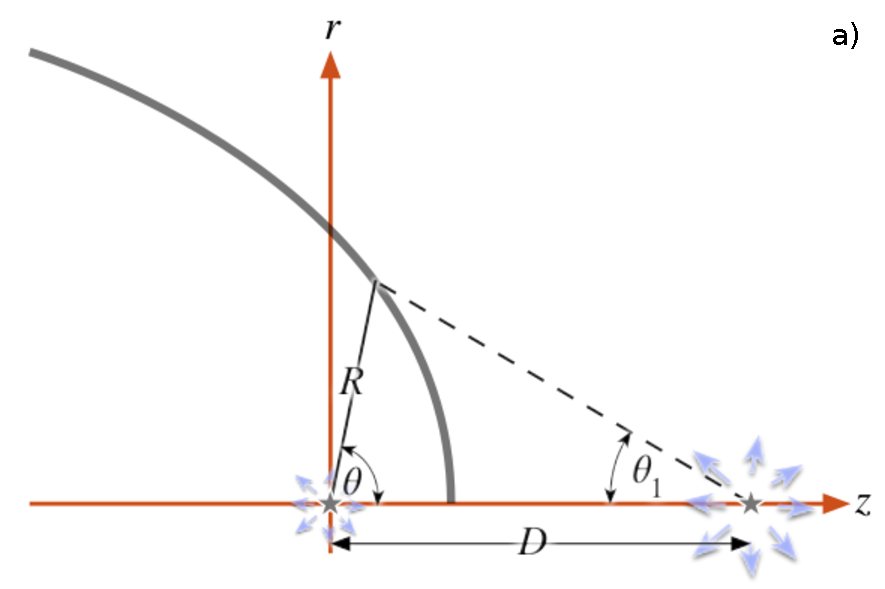
\includegraphics[width=\linewidth]{../Figures/bowshock-crw-variables}}
  \end{block}
  
}
\frame[label=Pi-Lambda]{\frametitle{Planitude and Alatude}
  \small
  \twocols{\begin{block}{}
      To characterize the shape of a given bow shock we use a set of parameters:
      \begin{itemize}
      \item \textbf<2>{The radius at the apex, called $R_0$, which gives us the bow shock physical scale, and is defined as the minimum of $R(\theta)$}
      \item \textbf<3>{The assymptotic angle $\theta_\infty$ of the far wings (which usually is not measurable)}
      \item \textbf<4>{The planitude $\Pi\equiv R_c/R_0$, which measures how flat is the apex}
        \item \textbf<5>{The alatude $\Lambda\equiv R_{90}/R_0$, which measures how open the wings are}
      \end{itemize}
      
    \end{block}}{\begin{block}{}\includegraphics<1>[width=\linewidth]{../Figures/characteristic-radii}
      \includegraphics<2>[width=\linewidth]{../Figures/characteristic-radii-r0}
      \includegraphics<3>[width=\linewidth]{../Figures/characteristic-radii-thinf}
      \includegraphics<4>[width=\linewidth]{../Figures/characteristic-radii-Pi}
      \includegraphics<5>[width=\linewidth]{../Figures/characteristic-radii-Lambda}
    \end{block}}
\hyperlink<4-5>{planitude}{\beamergotobutton{To see the algebraic expressions, click HERE}}
}
\frame{\frametitle{Winds Properties}
  \begin{block}{}
    \twocols{
    The relevant parameters of the winds are the terminal velocity $v$ and the mass loss rate $\dot{M}$, related to the density $\rho$. Following \citep{Canto:1996}, we use the sub-index $w$ for the weaker wind properties and the sub-index $w1$ for the stronger wind properties. }{\includegraphics[width=\linewidth]{../Figures/schematic-wind}}
  \end{block}}
\frame{\begin{block}{}
    And the winds momentum ratio, called $\beta$ (also following \citet{Canto:1996}) is given by:
      \begin{align*}
        \beta = \frac{\dot{M}^0_{w}v_{w}}{\dot{M}^0_{w1}v_{w1}}
      \end{align*}
      And is related with $R_0$ as follows:
      \begin{align*}
        \frac{R_0}{D} = \frac{\beta^{1/2}}{1+\beta^{1/2}}
      \end{align*}    
  \end{block}
  }

\frame{\frametitle{Quadrics of Revolution}
  \twocols{\begin{block}{}
      Quadrics of Revolution are the surfaces of revolution of conic sections. May be a good and useful approximation to more complex surfaces
    \end{block}}{\begin{block}{}
      \includegraphics[width=\linewidth]{../Figures/Quadrics}
    \end{block}
  }
}

\frame{\frametitle{Quadrics of Revolution: basic definitions}
  \begin{block}{}
    Our conic section symmetry axis is aligned with the $x$ axis, and the center is displaced from the origin by distance called $x_0$. The physical scale of the conic section is set using the semi-major and semi-minor axis $a$ and $b$.
  \twocols{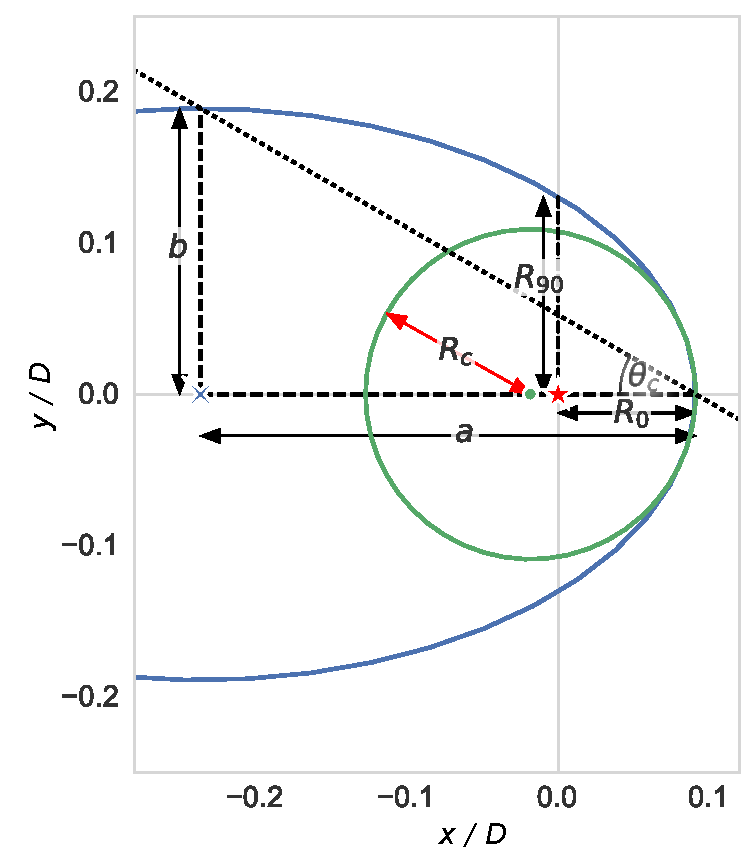
\includegraphics[width=0.7\linewidth]{../Figures/ellipse_edited}}
  {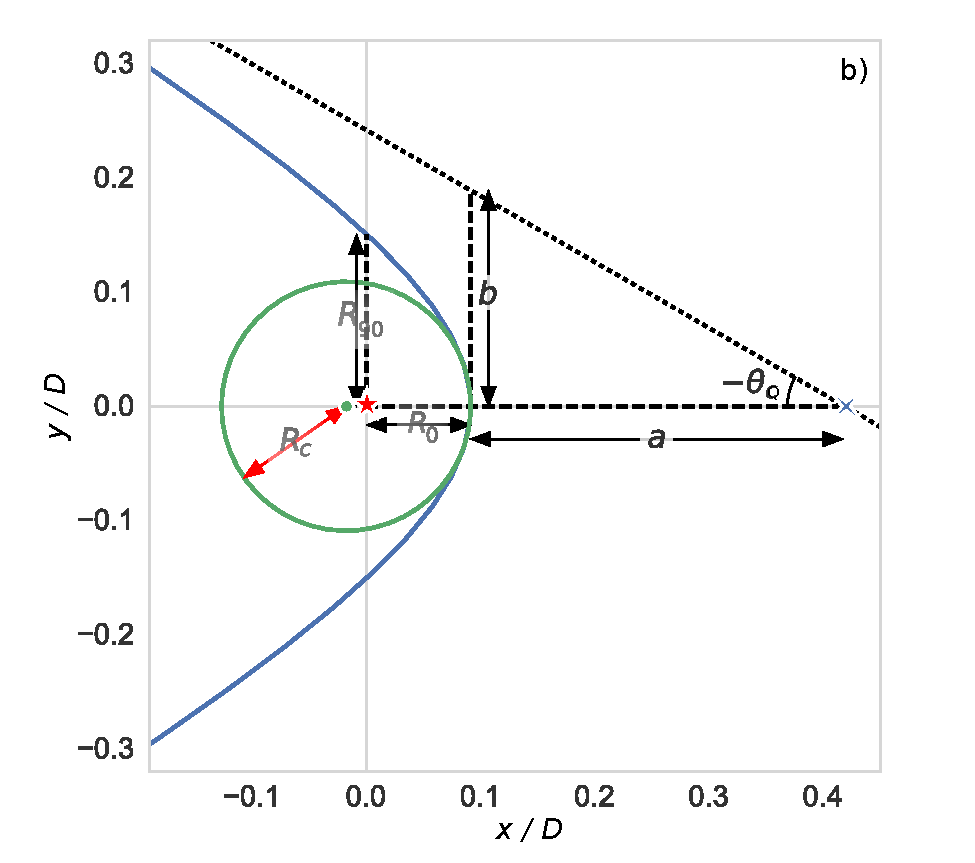
\includegraphics[width=\linewidth]{../Figures/hyperbola_edited}}
  \end{block}
}
\newcommand\Sin{\ensuremath{\mathcal{S}}}
\newcommand\Cos{\ensuremath{\mathcal{C}}}
\frame{\frametitle{Quadrics of Revolution: basic definitions}
  \twocols{\begin{block}{Parametrization}
      \footnotesize
      \begin{align*}
        x &= x_0 + \sigma a\Cos(t)\\
        y &= b\Sin(t) \\
        \tan\theta &= \frac{b\Sin(t)}{x_0 + \sigma a\Cos(t)}\\
        R &= \left[\left(x_0 + \sigma a\Cos(t)\right)^2 + b^2\Sin^2(t)\right]^{1/2}
      \end{align*} 
    \end{block}}{\begin{block}{where:}
      \footnotesize
      \begin{align*}
        t ~&\forall~ \mathbb{R} \\
  \Cos(t), \Sin(t) &=\left\lbrace
  \begin{array}{lr}
    \cos{t}, \sin t & \mathrm{ellipses}\\
    \cosh{t}, \sinh{t} & \mathrm{hyperbolas}       
  \end{array}\right. \\
  \sigma &= \left\lbrace
  \begin{array}{lr}
    +1 & \mathrm{ellipses} \\
    -1 & \mathrm{hyperbolas}
  \end{array}\right. \\
        x_0 &= R_0 -\sigma a %\label{eq:x0}
      \end{align*}
    \end{block}}
}
\newcommand\Q{\ensuremath{\mathcal{Q}}}
\frame{\frametitle{Quadrics of Revolution: basic definitions}
  \twocols{\begin{block}{}
      The eccentricity is replaced with the quadrics parameter \Q{} defined as:
      \begin{align*}
        \Q = \sigma\frac{b^2}{a^2}
      \end{align*}
      Or the angle $\theta_q$:
      \begin{align*}
        \tan\theta_q = \sigma\frac{b}{a}
      \end{align*}
      Positive values of \Q{} are associated with closed curves (i.e. ellipsoids), and $\Q \leq 0$ are associated with open curves.
    \end{block}}{\begin{block}{}
      \includegraphics[width=\linewidth]{../Figures/conic2}
    \end{block}}
}
\frame{\frametitle{Quadrics of Revolution: basic definititions}
  \twocols{\begin{block}{}
      The parameters set $(a, x_0, \Q)$ is enough to characterize the curve, but for future applications the set $(R_0, \Pi, \Lambda)$ is more useful. So, the transformation between the two sets is given by:
    \end{block}}{\begin{block}{}
      \begin{align*}
        R_0 &= x_0 + \sigma a \\
        \Pi &= \frac{a\Q}{a + \sigma x_0} \\
        \Lambda &= \left(\Q \frac{a - \sigma x_0}{a + \sigma x_0}\right)^{1/2}
      \end{align*}
    \end{block}}
  \begin{block}{}
    Finally, the quadrics parameter (and thus the kind of quadric) may be computed from the planitude and alatude as follows:
    \begin{align*}
      \Q = 2\Pi - \Lambda^2
    \end{align*}
  \end{block}
  
}

\frame{\frametitle{Projection Onto the Plane of Sky}
\twocols{\begin{block}{}We consider two reference frames in cartesian coordinates: The non primed reference system, where the $x$ axis is aligned with the symmetry axis of the bow shock, is called the body frame. And the primed system, where the $-z$ axis points toward the observer, is called the observer frame. The $x$ and $x'$ axis forms an angle called \textit{inclination} and is denoted as $i$. \end{block}}{\begin{block}{}\includegraphics[width=\linewidth]{../Figures/inclination}\end{block}}
}

\frame{\frametitle{Projection Onto the Plane of Sky}
  \twocols{
    \begin{block}{}
      The ``tangent line'' (the edge) of a bidimensional surface geometrically thin and optically thin is visible through limb brightening as an arc. The shape of the visible arc under these conditions varies with the inclination.
    \end{block}
  }{\begin{block}{}
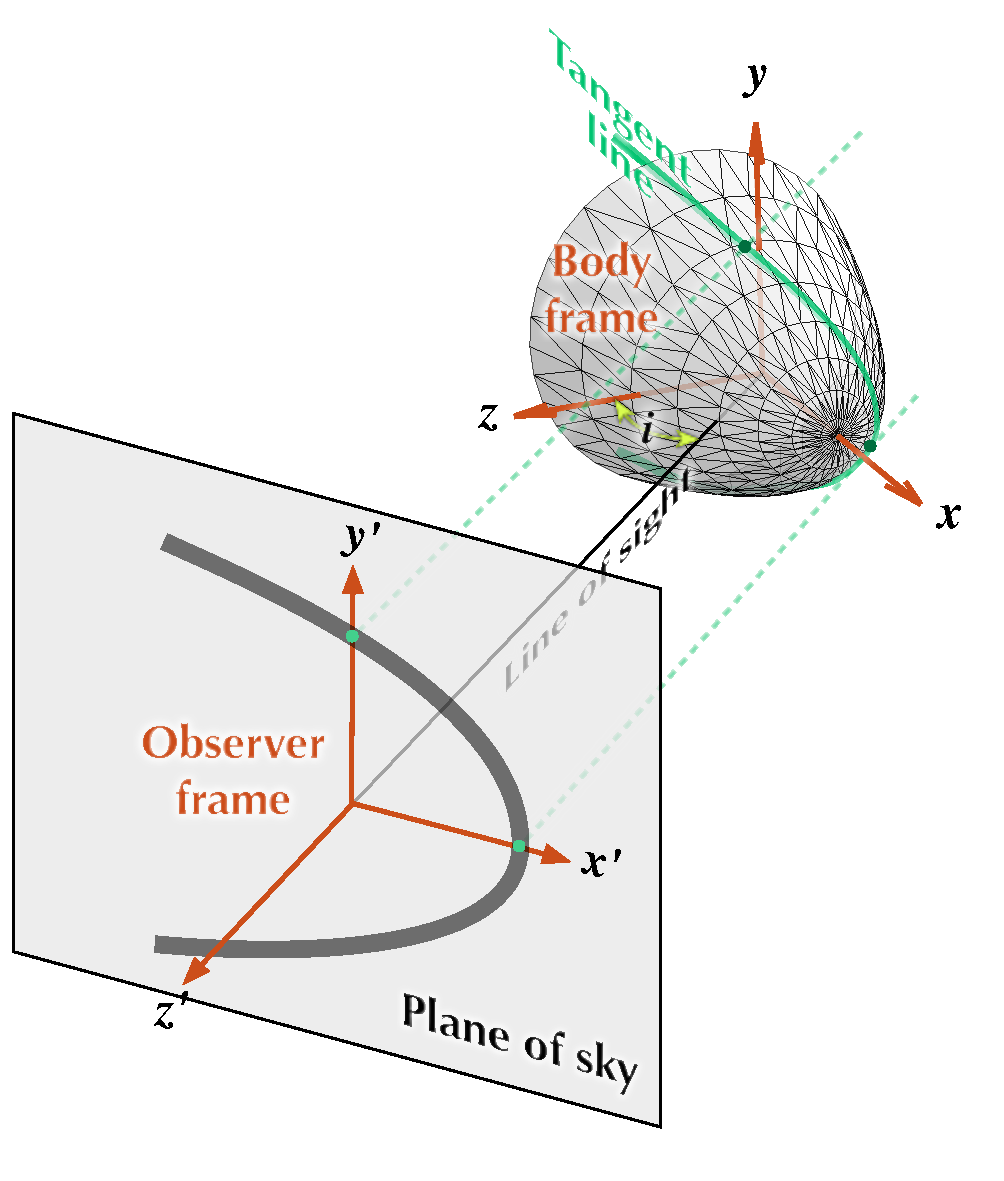
\includegraphics[width=\linewidth]{../Figures/projection-pos}
    \end{block}}
}

\frame[label=3d-shape]{\frametitle{Projection Onto the Plane of Sky}
  \begin{block}{Tridimensional shape in the body frame: Rotation along the $x$ axis of the bidimensional curve.}
    \includegraphics[width=\linewidth]{../Figures/projection-3d-shape-eq} \\
    \hyperlink{matrices}{\beamergotobutton{Go to Matrix Expression}}
  \end{block}
}

\frame[label=rot-matrix]{\frametitle{Projection Onto The Plane of Sky}
  \begin{block}{Transformation between body frame and observer frame}
    \includegraphics[width=\linewidth]{../Figures/projection-rotation-eq} \\
    \hyperlink{matrices}{\beamergotobutton{Go to Matrix Expression}}
  \end{block}  
}
\frame[label=tangent-line]{\frametitle{Projection Onto the Plane of Sky}
  \twocols{\begin{block}{Normal and tangent unit vectors}
      We define the unit vectors $\hat{t}$ and $\hat{n}$ as the tangent and normal vectors to the surface at certain point (to check the expression of each one go to \hyperlink{unit-vec}{\beamergotobutton{this slide}}). The tangent line of the surface at the inclination $i$ is such that the next condition is fullfilled:
      \begin{align*}
        \hat{n}\cdot\hat{z}' = 0
      \end{align*}
    \end{block}}{\begin{block}{}
      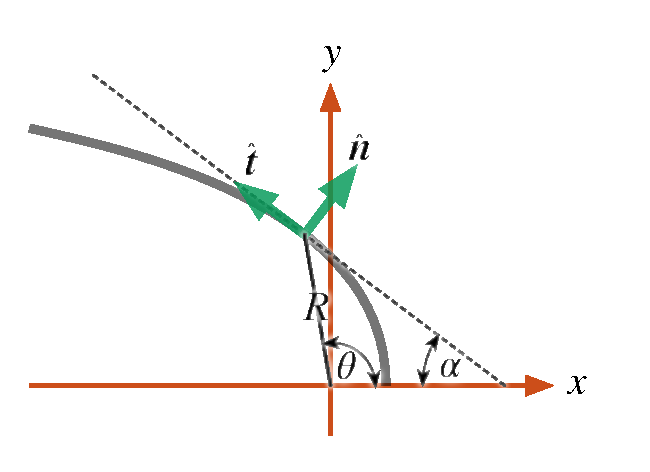
\includegraphics[width=\linewidth]{../Figures/bowshock-unit-vectors}
    \end{block}}
}
\frame{\frametitle{Projection Onto the Plane of Sky}
  \twocols{\begin{block}{}
      The angle $\phi$ which fulfills the tangent line condition is such that:
      \begin{align*}
        \sin\phi_T = \tan i~\frac{1 + \omega\tan\theta}{\omega-\tan\theta}
      \end{align*}
      where:
      \begin{align*}
        \omega = \frac{1}{R}\frac{dR}{d\theta}
      \end{align*}
    \end{block}
  }{\begin{block}{}
      With this, the projected shape is given by: \\
	  \includegraphics[width=\linewidth]{../Figures/projection-3d-shape-final-eq}
    \end{block}}
    \begin{block}{}
	    Since $z'_T$ is not constant, then the projected shape does not lie in a plane.
    \end{block}
}

\frame{\frametitle{Projected Alatude and Planitude}
\begin{block}{}
	For an arbitraty inclination, the tangent line does not exist for $\theta < \theta_0$, where:
\begin{align*}
	\tan\theta_0 = \frac{|\tan i| + \omega(\theta_0)}{1 - \omega(\theta_0)|\tan i|}
\end{align*}
For ``open'' shapes, when $i$ is large enough, there is no tangent line for any $\theta$.
\end{block}
\begin{block}{}
	The projected radius at the apex $R'_0$ is computed as $x'_T$ such that $y'_T=0$:
	\begin{align*}
		R'_0 = R(\theta_0)\cos(\theta_0 - |i|)
	\end{align*}
\end{block}}

\frame{\frametitle{Projected Alatude and Planitude}
\twocols{\begin{block}{}$R'_{90}$ is computed as $y'_T$ such that $x'_T=0$:
	\includegraphics[width=\linewidth]{../Figures/projection-3d-R90-eq}\\
	Where:\\
	\includegraphics[width=\linewidth]{../Figures/projection-3d-t90-eq}\\
	Finally $\Lambda = R'_{90}/R'_0$
\end{block}}{\begin{block}{}
	The apparent planitude is computed as the intrinsic planitude but in the observer frame:\\
	\includegraphics[width=\linewidth]{../Figures/projection-3d-planitude-eq}
\end{block}}
}

\newcommand\fQi{\ensuremath{f_{\scriptscriptstyle \Q, i}}}
\frame[label=proj-shape-quad]{\frametitle{Projected Shape of Quadrics of Revolution}
\twocols{\begin{block}{In terms of $(a, b, t)$}
	\includegraphics[width=\linewidth]{../Figures/projection-quad-shape-final-eq}
\end{block}}{\begin{block}{In terms of $(a', b', t')$}
	\begin{align*}
		x'_T &= a'\Cos(t') + x'_0\\
		y'_T &= b'\Sin(t')
	\end{align*}
\end{block}}
\twocols{\begin{block}{Where:}
	\begin{align*}
		a' &= a\cos i~\fQi \\
		b' &= b \\
		\Cos(t') &= \fQi\Cos(t)\\
		\fQi &= \left(1 + \Q\tan^2i\right)^{1/2}
	\end{align*}
\end{block}}{\begin{block}{}
	With this we show that the projected shape of a quadric is another quadric of the same type. The particular case of the paraboloid is shown \hyperlink{paraboloid}{\beamergotobutton{HERE}}.
\end{block}}
}

\frame{\frametitle{Projected Alatude and Planitude of Quadrics of Revolution}
\twocols{\begin{block}{Projected apex radius}
	\begin{align*}
		R'_0/R_0 = \cos i\left[1 + \frac{\Pi}{\Q}(1-\fQi)\right]
	\end{align*}
\end{block}}{\begin{block}{}
	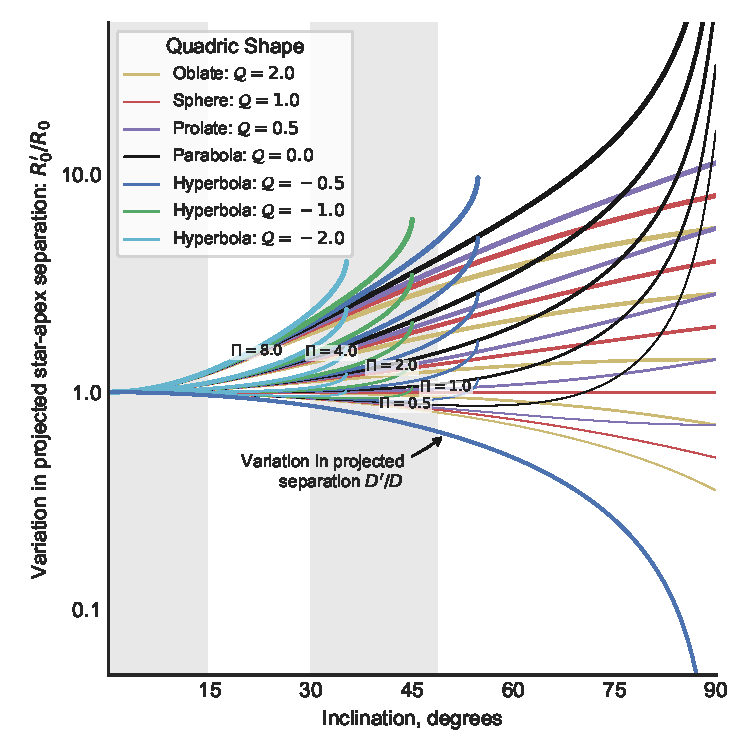
\includegraphics[width=\linewidth]{../Figures/projected-R0-vs-i}
\end{block}}
}

\frame{\frametitle{Projected Alatude and Planitude of Quadrics of Revolution}
\twocolspic{\begin{block}{Projected Planitude}
	\begin{align*}
		\Pi' = \frac{\Pi}{(R'_0/R_0)\fQi\cos i}
	\end{align*}
\end{block}}{\begin{block}{}
	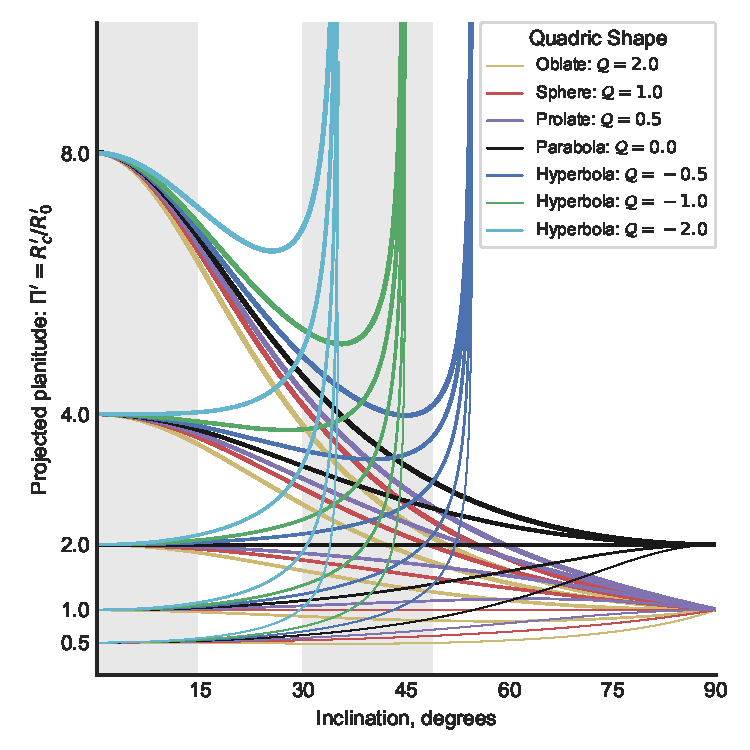
\includegraphics[width=\linewidth]{../Figures/projected-Rc-vs-i}
\end{block}}
}
\frame{\frametitle{Projected Alatude and Planitude of Quadrics of Revolution}
\twocolspic{\begin{block}{Projected Alatude}
	\begin{align*}
		\Lambda' = \left(2\Pi' - \Q'\right)^{1/2}
	\end{align*}
	where:
	\begin{align*}
		\Q' = \frac{\Q}{\fQi\cos^2i}
	\end{align*}
	\includegraphics[width=\linewidth]{../Figures/footnote}
\end{block}}{\begin{block}{}
	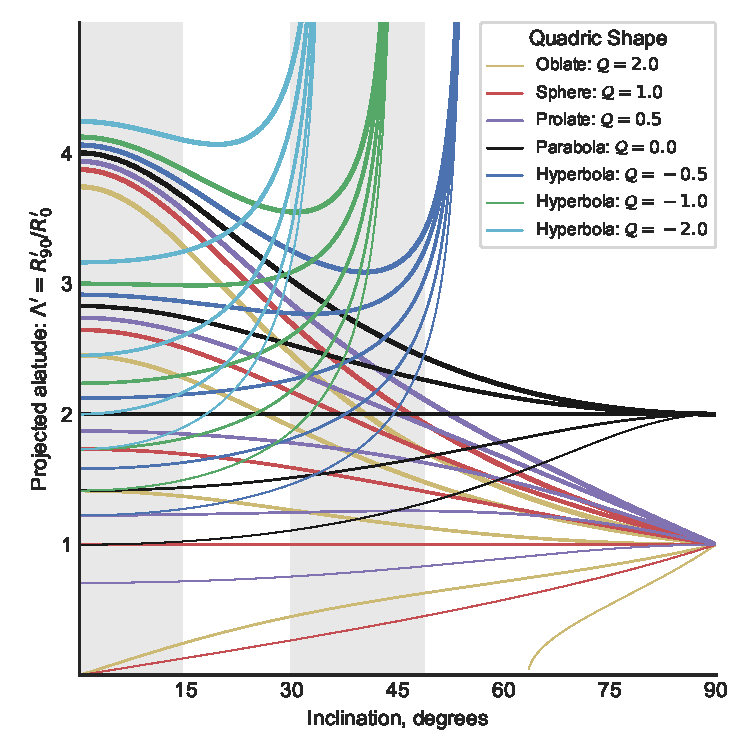
\includegraphics[width=\linewidth]{../Figures/projected-R90-vs-i}
\end{block}}
}

\frame{\frametitle{The $\Lambda-\Pi$ Diagram}
\twocolspic{\begin{block}{}
	\only<1-4>{Comparing the projected alatude against the projected planitude we identify three regions:}
	\begin{itemize}
		\only<2>{\item The upper region where the hyperboloid shapes lie.}
		\only<3>{\item A narrow intermediate region for the prolate ellipsoids.}
		\only<4>{\item The lower region for the oblate ellipsoids.}
	\end{itemize}
	\only<5>{The interfaces between regions correspond to the paraboloid and the spheroid.}
\end{block}}{\begin{block}{}
	\includegraphics<1>[width=\linewidth]{../Figures/projected-R90-vs-Rc}
	\includegraphics<2>[width=\linewidth]{../Figures/projected-R90-vs-Rc-3}
	\includegraphics<3>[width=\linewidth]{../Figures/projected-R90-vs-Rc-2}
	\includegraphics<4>[width=\linewidth]{../Figures/projected-R90-vs-Rc-1}
	\includegraphics<5>[width=\linewidth]{../Figures/projected-R90-vs-Rc-4}
\end{block}}
}
\section{Thin Shell Model}
\frame{\frametitle{Introduction}
\begin{block}{}
	A (little) more realistic model to compute the shape of the bow shock come from steady state hydrodinamical models for two winds interaction in the thin shell limit in stationary state. For example \citet{Canto:1996}. \\
	\centering
	\includegraphics[width=0.8\linewidth]{../Figures/CRW-abstract}
\end{block}
}
\frame[label=winds]{\frametitle{Winds symmetry}
\only<1>{\begin{block}{}
	The symmetry of the winds is classified into three scenarios:

	\textbf{Cantoid bow shocks}
\end{block}}
\only<2>{\textbf{Wilkinoid bow shocks}}
\only<3>{The previous two scenarios were discussed previously in \citet{Canto:1996}, but we add a third scenario:

\textbf{Ancantoid bow shocks}}

\twocols{\only<1-2>{\begin{block}{Isotropic inner wind}
	\centering
	\includegraphics[width=0.6\linewidth]{../Figures/anisotropic-arrows-1}
\end{block}}
\only<3>{\begin{block}{Anisotropic hemispherical wind}
	\small The density of the inner wind is proportional to $\cos^k\theta$, where $\theta$ is the polar angle and $k$ is the power index.
	$\mathbf{k=0}$.\\
	\includegraphics[width=0.6\linewidth]{../Figures/anisotropic-arrows-2}
\end{block}}
\only<4>{\begin{block}{Anisotropic hemispherical wind}
	$\mathbf{k=1/2}$, adequated for \hyperlink{bertoldi}{\beamergotobutton{proplyds}}.\\
	\includegraphics[width=0.6\linewidth]{../Figures/anisotropic-arrows-3}
\end{block}}
\only<5>{\begin{block}{Anisotropic hemispherical wind}
	$\mathbf{k=3}$.\\
	\includegraphics[width=0.6\linewidth]{../Figures/anisotropic-arrows-4}
\end{block}}

}{\only<1>{\begin{block}{Isotropic outer wind}
	\centering
	\includegraphics[width=0.6\linewidth]{../Figures/anisotropic-arrows-1}
\end{block}}
\only<2>{\begin{block}{Plane--parallel stream}
	\includegraphics[width=0.6\linewidth]{../Figures/plane-parallel}
\end{block}}
\only<3-5>{\begin{block}{Isotropic outer wind}
	\centering
	\includegraphics[width=0.6\linewidth]{../Figures/anisotropic-arrows-1}
\end{block}
}
}
	}
\frame[label=shape]{\frametitle{Discontinuity Contact Shape}
  \twocols{\begin{block}{}
	  \small
      The shape of the dicontinuity contact $R(\theta)$ is given by equation (6) of \citep{Canto:1996}:\\
      \includegraphics[width=\linewidth]{../Figures/eq-6-CRW} \\
	  Where the algebraic form of these quantities for the ancantoid inner winds (without the ``1'' suffix) are described \hyperlink{integrals}{\beamergotobutton{HERE}. For the outer winds (suffix ``1'') (equations (12-15) and (19-22) of \citet{Canto:1996} click \hyperlink{outer-wind}{\beamergotobutton{HERE}}) and for the inner wind for the cantoid and wilkinoid case (equations (8-11) of \citet{Canto:1996}, click \hyperlink{cantoid-int}{\beamergotobutton{HERE}}}
    \end{block}}{\begin{block}{}
      \includegraphics[width=\linewidth]{../Figures/momentum} \\
    \end{block}}
}
\frame{\frametitle{Discontinuity Contact Shape}
\twocols{\begin{block}{}
	An alternative form to get R is applying the sines law to the next triangle:
	\begin{align*}
		R = \frac{D\sin\theta_1}{\sin(\theta+\theta_1)}
	\end{align*}
\end{block}}{\begin{block}{}
	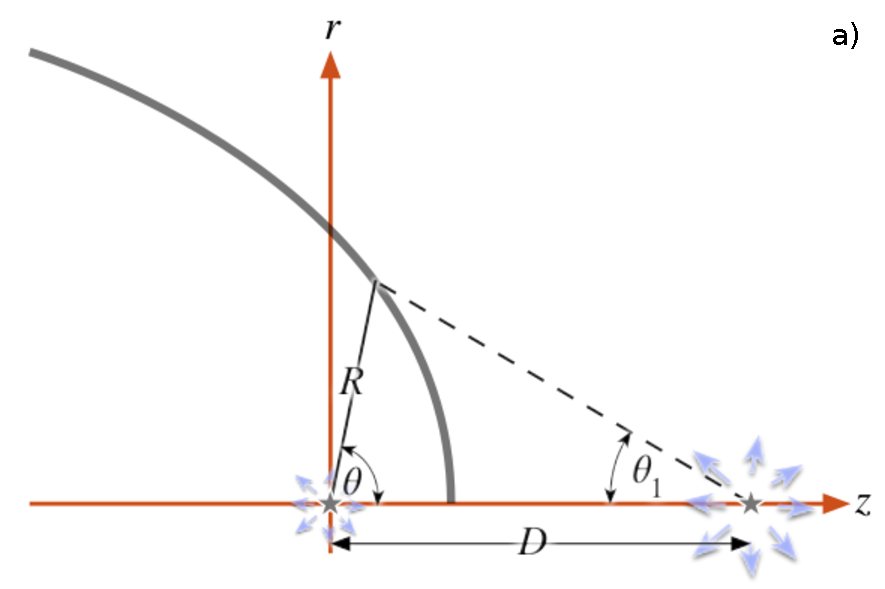
\includegraphics[width=\linewidth]{../Figures/bowshock-crw-variables}
\end{block}}
}
\frame{\frametitle{Discontinuity Contact Shape}
\twocols{\begin{block}{}
	With this, we get trascendent equations for $\theta_1$. Then solve for $\theta_1(\theta)$ and finally get R:
\end{block}
\begin{block}{Solution for Wilkinoids}
	\footnotesize
	For wilkinoids there is an explicit solution for $R(\theta)$:
	\begin{align*}
		R = R_0\left[\csc^2\theta(1-\theta\cot\theta)\right]^{1/2}
	\end{align*}
	Where:
	\begin{align*}
		R_0 = \left(\frac{\dot{M}_w^0v_w}{4\pi\rho_av_a^2}\right)^{1/2}
	\end{align*}
	Where $\rho_a$ and $v_a$ are the density and velocity of the plane--parallel outer wind
\end{block}}{\begin{block}{For Cantoids}
	\includegraphics[width=\linewidth]{../Figures/cantoid-t1-t}
\end{block}
	\begin{block}{For ancantoids head}
		\includegraphics[width=\linewidth]{../Figures/ancantoid-t1-t}
	\end{block}
\begin{block}{For ancantoids tail}
	\includegraphics[width=\linewidth]{../Figures/ancantoid-t1-t-tail}
\end{block}}
}
\frame{\frametitle{Discontinuity Contact Shape}
Where:
\twocols{\begin{block}{Ancantoids}
	\footnotesize
	\begin{align*}
		\beta = 2(k+1)\frac{\dot{M}_w^0v_w}{\dot{M}_{w1}^0v_{w1}}
	\end{align*}
\end{block}}{\begin{block}{Cantoids}
	\footnotesize
	\begin{align*}
		\beta = \frac{\dot{M}_w^0v_w}{\dot{M}_{w1}^0v_{w1}}
	\end{align*}
\end{block}}
\twocols{\begin{block}{Fixed $\beta$}
	\includegraphics[width=\linewidth]{../Figures/cantoid-ancantoid-shape-bfixed}
\end{block}}{\begin{block}{Fixed $k$}
	\includegraphics[width=\linewidth]{../Figures/ancantoid-shape}
\end{block}}
}
\frame{\frametitle{Planitude and Alatude}
\twocols{\begin{block}{Planitude}
	\only<1>{Ancantoids:
	\begin{align*}
		\Pi = \left|1-2\frac{R_{\theta\theta, 0}}{R_0}\right|^{-1}
	\end{align*}
	Where:
	\begin{align*}
		R_{\theta\theta, 0} &= \frac{C_{k\beta}}{1+\beta^{1/2}} + \frac{1+2\beta^{1/2}}{3} \\
		C_{k\beta} &= \frac{1}{15} - \frac{3k}{20} - \frac{\beta}{15}
	\end{align*}}
	\only<2-3>{
		Cantoids:
		\begin{align*}
			\Pi = \frac{5}{3\left(1-\beta^{1/2}\right)}
		\end{align*}}
	\only<3>{Wilkinoids:
	\begin{align*}
		\Pi = \frac{5}{3}
	\end{align*}}
\end{block}}{\begin{block}{Alatude}
	\only<1>{Ancantoids:
	\begin{align*}
		\Lambda = \frac{\left(3\xi\right)^{1/2}(1+\beta^{1/2})}{\left(1+\frac{1}{5}\xi\beta\right)^{1/2}(1-\xi\beta)}
	\end{align*}
	Where:
	\begin{align*}
		\xi = \frac{2}{k+2}
	\end{align*}}
	\only<2-3>{Cantoids:
	\begin{align*}
		\frac{\sqrt{3}}{\left(1+\frac{1}{5}\beta\right)^{1/2}\left(1-\beta^{1/2}\right)}
	\end{align*}}
	\only<3>{Wilkinoids:
	\begin{align*}
		\Lambda = \sqrt{3}
	\end{align*}}
\end{block}}
}
\frame{\frametitle{Planitude and Alatude}
\twocols{\begin{block}{}
	\begin{align*}
		\Pi &= \frac{5}{3} \\
		\Lambda &= \sqrt{3}  
	\end{align*}
	Is to note that the Wilkinoid case works as the assymptotic limit of cantoids when $\beta\to 0$
\end{block}}{\begin{block}{}
	\includegraphics[width=\linewidth]{../Figures/cantoid-wilkinoid-shape}
\end{block}}
}
\frame{\frametitle{Thin Shell model fits to quadrics of Revolution}
\twocols{\begin{block}{}
	\only<1>{Once computed the planitude and alatude, we may estimate the quadrics parameter $\Q$ or the equivalent $\theta_Q$ which approximates the shape of the bow shock head. As well the assymptotic angle $\theta_\infty$ is used to estimate the same parameters for the bow shock tail.}
	\only<2>{For a wide range of the anisotropy parameter $k$, for low $\beta$ values the shape of the head fits with an ellipsoid and for higher $\beta$ the head fits better with an hyperboloid. While the tail always fits with an hyperboloid. This will help us to understand the behavior of the apparent shape in a $\Lambda-\Pi$ diagram.}
\end{block}}{\begin{block}{}
	\includegraphics[width=\linewidth]{../Figures/ancantoid-angles}
\end{block}}
}
\frame{\frametitle{Projected Planitude and Alatude}
	\twocols{\begin{block}{}
		\only<1>{The apparent shape of multiple types of bow shocks becomes more open as the inclination increases. Because the tangent line shifts to the hyperbolic part of the bow shock (the tail) as the inclination increases.}
		\only<2>{The wilkinoid is the exception of the rule (shape becomes closer with inclination). The confocal paraboloid $(\Pi=\Lambda=2)$ does not change with inclination (another shape not mentioned here is the trivial case of the confocal spheroid $(\Lambda=\Pi=1)$).}
	\end{block}}{\begin{block}{}
		\includegraphics<1>[width=\linewidth]{../Figures/ancantoid-apparent-shape}
		\includegraphics<2>[width=\linewidth]{../Figures/cantoid-apparent-shape}
	\end{block}}
}

\frame[label=thin-shell-diagram]{\frametitle{Projected Planitude and Alatude: $\Lambda-\Pi$ diagram}
\twocols{\begin{block}{Main notes}
	\only<1>{The circle shows the shape of the bow shock in the body frame $(i=0)$ and the inclination grows along the curve. For low $\beta$ the apparent shape changes from ellipsoid to hyperboloid.}
	\only<2>{The ancantoids show a ``kink'' at an inclination shuch that the apparent apex passes through the inner wind discontinuity, where the second derivative of $R(\theta)$ has a slope deviation. This kink softens as the anisotropy parameter increases. \hyperlink{2-derivative}{\beamergotobutton{Click HERE}}}
	\only<3>{The wilkinoid track does not show sustancial variations.}
\end{block}}{\begin{block}{}
	\includegraphics<1>[width=\linewidth]{../Figures/ancantoid-R90-vs-Rc-a}
	\includegraphics<2>[width=\linewidth]{../Figures/ancantoid-R90-vs-Rc-b}
	\includegraphics<3>[width=\linewidth]{../Figures/ancantoid-R90-vs-Rc-lobeta-a}

\end{block}}
}

\section{Results Obtained for the Classical Proplyds in Orion Nebula}
\frame{\frametitle{The Trapezium observed with the HST}
\includegraphics[width=\linewidth]{../Figures/Trapezium-annotate-rob-2018}
}

\frame{\frametitle{Obtaining the data}
\twocols{With DS9 tools, we get the coordinates (AR, DEC) of each proplyd (small circles), the position of \thC{} (red cross) and the position of each bow shock (cyan crosses).}{\begin{block}{}
	\includegraphics[width=\linewidth]{../Figures/Trapezium-annotate-rob-2018}
\end{block}}
}
\frame{\frametitle{Obtaining the data}
\twocols{\begin{block}{}
	\only<1>{For each proplyd we measured the radius of curvature with a circular least square fit of the bow shock marks. $R_0$ is measured along the line between the proplyd and $\thc{}$ from the proplyd position to the resultant circle. And obtain with this the planitude. The alatude is not available for any proplyd in the sample.}
	\only<2>{The number and spacing of the marks are proportional to the size of the bow shock and to our confidence in that we are tracing the bow shock correctly.}
\end{block}
\only<2>{\begin{block}{169-338}
	\includegraphics[width=\linewidth]{../Programs/LV-bowshocks-xyfancy-positionswill-169-338}
\end{block}}
}{\begin{block}{\only<2>{177-341}}
	\includegraphics<1-2>[width=\linewidth]{../Programs/LV-bowshocks-xyfancy-positionswill-177-341}
\end{block}}
}
\frame{\frametitle{Sub-samples}
\twocols{\begin{block}{}
	For each proplyd, we did a set of sub-samples where we removed randomly about $1/3$ of the marks (but left at least 4) and measure the planitude for each sub-sample. The deviation between sub-samples and the ``main'' measurement (without removing marks) measures the uncertainties of both the apparent apex radius and planitude. 	
\end{block}}{\begin{block}{\only<1>{Main}\only<2-4>{Sub-sample example}}
	\includegraphics<1>[width=\linewidth]{../Programs/LV-bowshocks-xyfancy-positionswill-168-328}
	\includegraphics<2>[width=\linewidth]{../Programs/Multi-Fit/samp00/LV-bowshocks-xyfancy-positionssamp00-168-328}
	\includegraphics<3>[width=\linewidth]{../Programs/Multi-Fit/samp02/LV-bowshocks-xyfancy-positionssamp02-168-328}
	\includegraphics<4>[width=\linewidth]{../Programs/Multi-Fit/samp04/LV-bowshocks-xyfancy-positionssamp04-168-328}
\end{block}}
}

\frame{\frametitle{$\Pi-R_0/D$ diagram}
\twocols{\begin{block}{}
	\only<1>{Since the alatude is not available for our set, we compare all the results in a $\Pi-R_0/D$ diagram against the thin shell model predictions, assuming a given anisotropy index $k$.}
	\only<2>{For each proplyd, we may find multiple predictions for the winds momentum ratio $\beta$ and inclination $i$ for a given anisotropy index $k$ by examining the intersections between the observations (black dots with radial uncertainty bars) and the thin shell model predictions (each curve has a fixed value of $\beta$ and the inclination increases from left to right along each curve. Fixed intervals of $i$ in degrees are shown).}
	\only<3>{Each set of the parameters $(k, \beta, i)$ allows to estimate the intrinsic distance $D$ and the intrinsic apex radius $R_0$.}
\end{block}}{\begin{block}{}
	\includegraphics<1>[width=\linewidth]{../Figures/obs-diagnostic-Pi-R0-Cantoid}
	\includegraphics<2>[width=\linewidth]{../Figures/obs-diagnostic-Pi-R0-k05}
	\includegraphics<3>[width=\linewidth]{../Figures/obs-diagnostic-Pi-R0-k30}
\end{block}}
}
\frame[label=i-balance]{\frametitle{Ionization and ram pressure balance}
\begin{block}{}
	Having the true distance $D$ estimated, we may evaluate ionization equilibrium in the photoevaporated flux.
\end{block}
\twocolspic{\begin{block}{Ionization equilibrium condition}
	\small
	\begin{align*}
		F_* = u_{IF}n_{IF} + \omega r_{IF}\alpha'_{rec}n_{IF}^2
	\end{align*}
\end{block}
\begin{block}{Ionizing flux from the star.}
	\begin{align*}
		F_* = \frac{(1-f_d)\mathcal{N}_*}{4\pi D^2}
	\end{align*}
\end{block}
}{\begin{block}{}
	\includegraphics[width=\linewidth]{../Figures/ionization-balance}
\end{block}}
}

\frame{\frametitle{Ionization and ram pressure balance}
\twocols{\begin{block}{Inner wind pressure in the shell.}
	\begin{align*}
		P_{in} = \rho_{ps}v_w^2
	\end{align*}
\end{block}
\begin{block}{Star's ram pressure}
	\begin{align*}
		P_*(r) = \frac{\dot{M}_{w1}v_{w1}}{4\pi r^2}
	\end{align*}
\end{block}}{\begin{block}{}
	\includegraphics[width=\linewidth]{../Figures/pressure-equilibrium}
\end{block}}
}
\frame{\frametitle{\thC{} wind parameters}
\begin{block}{}
	For the outer wind coming from \thC{} we have the observational constrain \citep{Garcia-Arredondo:2001} that the ratio $\dot{M}_{-7}/v_3$ must be about 2. The two models which fullfill this condition are the following:
	\twocols{\begin{block}{\citep{GAH:2002}}
		\begin{align*}
			\dot{M}_{w1} &= \SI{3.5e-7}{M_\odot.yr^{-1}} \\
			v_{w1} &= \SI{1200}{km.s^{-1}}
		\end{align*}
		This model fullfills the aditional constrain that $\dot{M}_{-7}v_3 = 4.2$.
	\end{block}}{\begin{block}{\citep{Gagne:2005}}
		\begin{align*}
			\dot{M}_{w1} &= \SI{5.5e-7}{M_\odot.yr^{-1}}\\
			v_{w1} &= \SI{2760}{km.s^{-1}}
		\end{align*}
		These values are obtained with X-ray spectroscopy and MHD simulations.
	\end{block}}
\end{block}
}
\frame{\frametitle{Inner wind density}
\begin{block}{}
	For the inner wind density we compare two assumptions. In both cases, we use the ionization front radius reported by \citet{Garcia-Arredondo:2001} but corrected  by a factor of $\simeq 0.96$ due to the distance to orion nebula.
 \end{block}
 \twocols{\begin{block}{\small Importing ionization front densities from \citet{Garcia-Arredondo:2001}}
     \small
  \begin{tabular}{ccc} \toprule
    Source  & $r_{\mathrm{IF}, 14}$     & $N_6$ \\
    \midrule
    168-328   & $2.7 \pm 0.3$  & $4.08 \pm 0.48$ \\
    169-338   & $2.7 \pm 0.3$  & $1.43 \pm 1.09$ \\
    177-314   & $19.6 \pm 1.9$ & $0.42 \pm 0.06$ \\ 
    180-331   & $11.7 \pm 1.3$ & $0.49 \pm 0.08$ \\
    LV2       & $7.6 \pm 0.4$  & $2.65 \pm 0.23$ \\
    LV2b      & $2.4 \pm 0.6$  & $4.21 \pm 1.21$ \\
    LV3       & $4.8 \pm 0.7$  & $3.19 \pm 0.71$ \\
    LV4       & $3.4 \pm 0.3$  & $4.21 \pm 0.63$ \\
    LV5       & $6.1 \pm 0.7$  & $2.37 \pm 0.47$ \\
  \end{tabular}

\end{block}}{\begin{block}{\small Derivated from our estimations of $\beta$}
	\small
We may derive the pre shock wind density as follows:
	\begin{align*}
		n_{ps} = \frac{\beta\left(\dot{M}_{w1}v_{w1}\right)}{4\pi R_0^2\mu m_Hv_w^2}
	\end{align*}
	Where $\mu=1.3$ for a gas with a sound speed of $\simeq \SI{11}{km.s^{-1}}$. This assumption implies that pressure equilibrium is archived.
\end{block}}
}

\frame{\frametitle{Ionization balance and ram pressure equilibrium}
\twocols{\begin{block}{\only<1-2>{Importing inner wind densities from \citet{Garcia-Arredondo:2001}}\only<3-5>{Derivated inner wind density from estimations of $\beta$}}
	\only<1-2>{Finally, for the inner wind velocity $v_w$ we tried the range $M=[2,3]$, where $M$ is the Mach number of the inner wind: $M\equiv\frac{v_w}{c_{II}}$.}
	\only<3-4>{The gray line is the ram pressure of \thC{} obtained by \citet{Garcia-Arredondo:2001, GAH:2002}}
	\only<5>{The green line is the ram pressure of \thC{} obtained by \citet{Gagne:2005}}
	\only<6-7>{Finally, we compare with previous work \citep{HA:1998, Garcia-Arredondo:2001, Henney:2002}}
\end{block}\only<5>{\begin{block}{}
	Here we note how the ram pressure equilibrium assumption is accomplished.
\end{block}}}{\begin{block}{\only<1,3,6>{M=2}\only<2,4-5,7>{M=3}}
	\centering
	\includegraphics<1>[width=0.75\linewidth]{../Figures/plot-wind-fits-2}
	\includegraphics<2>[width=0.75\linewidth]{../Figures/plot-wind-fits}
	\includegraphics<3>[width=0.75\linewidth]{../Figures/plot-wind-fits-beta-2}
	\includegraphics<4>[width=0.75\linewidth]{../Figures/plot-wind-fits-beta}
	\includegraphics<5>[width=0.75\linewidth]{../Figures/plot-wind-fits-beta-Gagne}
	\includegraphics<6>[width=0.75\linewidth]{../Figures/plot-wind-fits-HA98-2}
	\includegraphics<7>[width=0.75\linewidth]{../Figures/plot-wind-fits-HA98}
\end{block}}
}
\section{Summary and Conclusions}

\frame{\frametitle{Summary and conclusions}
\begin{block}{}
	\small
\begin{itemize}
	\item The shape of an (ideally) cylindrically symmetric bow shock can be characterized by two adimensional parameters: the planitude $\Pi$ and the alatude $\Lambda$ that can be obtained from theoretical models (such as the thin shell model but not restricted to) or observations.
	\item We develop a general method to find the projected shape (i.e, the limb brightened edge) or tangent line, described with the parameters $(\Pi', \lambda')$, of a bow shock idealized as a cylindrical surface as a function of the inclination angle $i$.
	\item This method was applied to find inclination depending curves into the $\Lambda'-\Pi'$ plane for two sets of surfaces:
		\begin{itemize}
			\item \textbf{Quadric surfaces}, which are the surfaces of revolution of the conic sections.
			\item The solutions of the \textbf{Thin Shell Model} \citep{Canto:1996}
		\end{itemize}
	\item Open quadrics (hyperboloids) and close quadrics (ellipsoids) occupy different regions of the plane, and the interface between them is occupy by paraboloids. Any given curve does not move from one region to other.
\end{itemize}
\end{block}
}
\frame{\frametitle{Summary and conclusions}
\begin{block}{}
	\small
	\begin{itemize}{}
		\item In the $|i|\to 90^\circ$ limit, the apparent shape of all the ellipsoids tend to $\Pi'=\Lambda'=1$,the paraboloids tend to $\Pi'=\Lambda'=2$ and for the hyperboloids $(\Pi', \Lambda')\to(\infty, \infty)$ for a critical inclination $i_{crit}$ where the tangent line only exists for $|i| < i_{crit}$.
		\item This implies that the apparent shape of the confocal sphere $(\Pi=\Lambda=1)$ and paraboloid $(\Pi=\Lambda=2)$ is independent of inclination.
	\end{itemize}
\end{block}
}
\frame{\frametitle{Summary and Conclusions}
\begin{block}{}
	\begin{itemize}
		\item For the Thin Shell Model we found the inclination dependent curves for the shape of the discontinuty contact under three scenarios:
			\begin{itemize}
				\item A spherically symmetric, isotropic and non accelerated wind interacting with another spherically symmetric, isotropic and non accelerated wind. The resultant bow shock is called \textit{Cantoid}.
				\item A spherically symmetric, isotropic and non accelerated wind interacting with a plane -- parallel stream of constant velocity and density. The resultant bow shock is called \textit{Wilkinoid}.
				\item An spherically symmetric, anisotropic and non accelerated wind, where its density follows a power law of $\cos\theta$ interacts with a spherically symmetric, isotropic and non accelerated wind. The resultant bow shock is called \textit{Ancantoid}. 
			\end{itemize}
	\end{itemize}
\end{block}
}
\frame{\frametitle{Summary and Conclusions}
\begin{block}{}
	\begin{itemize}
		\item The shape of the discontinuity contact $R(\theta)$ of the wilkinoid shapes is fully characterized with the apex radius $R_0$. For the cantoids the shape is fully characterized with the winds momentum ratio $\beta$. And the ancantoids require additionally the anisotropy index $k$.
		\item The wilkioid shape acts as the limit of the cantoids when $\beta\to 0$.
		\item For low $\beta$ and regardless of $k$, the shape of the head fits to an ellipsoid and for higher values it fits better to an hyperboloid. This can be estimated calculating the planitude and alatude for a given $(k, \beta)$.
		\item The shape of the tail always fits with an hyperboloid, and can be estimated from the assymptotic angle $\theta_\infty$.
		\item The inclination dependent curves of the thin shell model solutions move from the prolate ellipsoid region to the hyperboloid region as the inclination increases (with the exception of the wilkinoid curve).
			\end{itemize}
\end{block}
}

\frame{\frametitle{Summary and Conclusions}
\begin{block}{}
	\begin{itemize}
		\item The inclination dependent curves of the ancantoids show a kink at an inclination such that the aparent apex passes through the point where the inner wind is cut off.
		\item We apply this work to the bow shocks observed in the core of the Orion Nebula due to the wind/wind interaction between proplyd's photoevaporated flow and \thC{} wind. 
		\item We measured the projected distance $D'$ to \thC{} for a set of proplyds and the projected planitude $\Pi'$ of their respective bow shock. The projected alatude was not measured due to the decay of emmision with $\theta$.
		\item We compared visually each measurement of planitude against the thin model predictions. Assuming a given anisotropy index $k$, we obtain may plausible values for the inclination and the winds momentum ratio $\beta$, leading us to estimate the intrinsic dimensions of each bow shock and the intrinsic distance to \thC{}.
	\end{itemize}
\end{block}
}

\frame{\frametitle{Summary and Conclusions}
\begin{block}{}
	\begin{itemize}
		\item Following the observational constriction $\dot{M}_{-7}/v_3 \simeq 2$ for the wind of \thC{} \citep{Garcia-Arredondo:2001}, we compared two models for this wind: $\dot{M}_{w1} = \SI{3.5e-7}{M_\odot.yr^{-1}}$ and $v_{w1}=\SI{1200}{km.s^{-1}}$ \citep{Garcia-Arredondo:2001, GAH:2002}. And $\dot{M}_{w1} = \SI{5.5e-7}{M_\odot.yr^{-1}}$ and $v_{w1}=\SI{2760}{km.s^{-1}}$ \citep{Gagne:2005}.
		\item We assume the inner wind velocity lies in the range $M=[2, 3]$, and for the density we may assume that ram pressure balance prevails, so we can derive the density from our estimations of $\beta$, and evaluate only the ionization balance condition. Or import the densities from \citet{Garcia-Arredondo:2001} and evaluate both conditions simultaneously.
	\end{itemize}
\end{block}
}
\frame{\frametitle{Future work}
\begin{block}{}
	\begin{itemize}
		\item For the Orion Nebula proplyds, improve methodology to obtain $\beta$ and inclinations in order to get a better resolution in the $(\beta, k, i)$ grid. 
		\item Improve methodology to evaluate balance conditions.
		\item Develop other models where bow shocks occur besides the thin shell model (Henney et al. in prep)
		\item Apply the techique developed in this work to other classes of stellar bow shocks: OB runaway stars \citep{Kobulnicky:2016} and red giant and supergiant stars \citep{Cox:2012}. And for LL objects in the outskirts of Orion Nebula \citep{Henney:2013}.
	\end{itemize}
\end{block}
}

\frame{
	\includegraphics[width=\linewidth]{../Figures/Thanks}
}
\frame[allowframebreaks]{\frametitle{References}
\bibliographystyle{mnras}
\bibliography{defense_biblio}
}

\frame{
  \begin{block}{MPAQ (Most Probably Asked Questions)}
    \centering
    \includegraphics[width=0.5\linewidth]{../Figures/just-in-case}
    \end{block}
}

\frame[label=Rob-image]{
  \begin{block}{}
    \centering
    \includegraphics[width=0.5\linewidth]{../Figures/Orion_Robberto}\\
    \footnotesize The trapezium region at \SI{10}{\mu.m} by \citet{Robberto:2005}
    \hyperlink{Robberto}{\beamergotobutton{Return Button}}
\end{block}
}
\frame[label=planitude]{\frametitle{Planitude and Alatude: Algebraic expressions}
	\twocols{\begin{block}{Planitude}
		\begin{align*}
			\Pi = \frac{R_0}{R_0 - R_{\theta\theta, 0}}
		\end{align*}
		Where $R_{\theta\theta,0}$ is the second derivative of $R$ at the apex.
	\end{block}}{\begin{block}{Alatude}
		\begin{align*}
			\Lambda = \frac{R(\pi/2)}{R_0}
		\end{align*}
	\end{block}}
	\hyperlink{Pi-Lambda}{\beamergotobutton{Return Button}}
}
\frame[label=matrices]{\frametitle{Useful Matrices}
  \centering
  \includegraphics[width=0.6\linewidth]{../Figures/projection-3d-mat-eq}\\
  \hyperlink{3d-shape}{\beamergotobutton{Return Button 1}}\\
  \hyperlink{rot-matrix}{\beamergotobutton{Return Button 2}}
}
\frame[label=unit-vec]{\frametitle{Useful unitary vectors}
  \begin{block}{}
    \centering
    \includegraphics[width=0.8\linewidth]{../Figures/projection-3d-vec-eq}\\
    \hyperlink{tangent-line}{\beamergotobutton{Return Button}}
  \end{block}
}


\frame[label=paraboloid]{\frametitle{Paraboloid}
\begin{block}{}
	In the parametric equations for the paraboloid, we assume that we know the planitude $\Pi$. \hyperlink{proj-shape-quad}{\beamergotobutton{Return Button}}
\end{block}
\twocolspic{\begin{block}{Intrinsic Shape}
	\begin{align*}
		x/R_0 &= 1 - \frac{1}{2}\Pi t^2\\
		y/R_0 &= \Pi t
	\end{align*}
\end{block}}{\begin{block}{Apparent shape in terms of $(t, \Pi)$}
	\includegraphics[width=\linewidth]{../Figures/projection-quad-shape-par-eq}
\end{block}}
\twocolspic{\begin{block}{Apparent shape in terms of $(t', \Pi')$}
		\begin{align*}
		x'_T/R'_0 &= 1 - \frac{1}{2}\Pi' t'^2\\
		y'_T/R'_0 &= \Pi' t'
		\end{align*}
\end{block}}{\begin{block}{where:}
	\centering
	\includegraphics[width=0.6\linewidth]{../Figures/projection-quad-shape-par-eq-2}
\end{block}}
}
\frame[label=bertoldi]{\frametitle{Anisotropy index for proplyds}
\twocolspic{\begin{block}{}
	\only<1>{Let us consider a globule of neutral gas irradiated by a plane--parallel ionizing radiation field from a distant source forming a ionization front and a photoevaporated flux of ionized gas.}
	\only<2>{A fraction of the incident flux is absorbed for recombined atoms (to all states except ground state) from the photoevaporated flux itself.}
	\only<3>{The ionizing flux that actually reaches the ionizing front and evaporates new material from the globule as a fuction of the polar angle $\theta$ is given by \citep{Bertoldi:1989}:
	\begin{align*}
		F_{II}(\theta) = F_{II}(0)\cos^{\ss}\theta
	\end{align*}
	Where:
	\begin{align*}
		\ss \simeq -\left(2 + \frac{1.53}{q-\phi_q}\right)^{-1}
	\end{align*}
	}
	\only<4>{$q$ is the ratio between the the ionizing radiation flux and the flux of ionized gas streaming off the the ionization front.
	
	And $\phi_q$ is a measure of the thickness of the ionization front.}
\end{block}}{\begin{block}{}
	\includegraphics<1>[width=\linewidth]{../Figures/bertholdi-cartoon-1}
	\includegraphics<2>[width=\linewidth]{../Figures/bertholdi-cartoon-2}
	\includegraphics<3>[width=\linewidth]{../Figures/bertholdi-cartoon}
	\includegraphics<4>[width=\linewidth]{../Figures/bertholdi-cartoon-3}
\end{block}}
}
\frame{\frametitle{Anisotropy index for proplyds}
\begin{block}{}
	\only<1>{The extreme case $q \gg 1$ implies that most of the incident radiation is absorbed when re-ionizing the recombining gas and only a small fraction reaches the ionizing front and ionizes the neutral gas. In this case we have a thin ionization front, so we have $\phi_q \simeq 1$. That implies that $\ss \simeq -1/2$. \\
	In the other extreme case $q \ll 1$ we have $q \simeq \phi_q$ that implies $\ss \simeq 0$.
}
	\only<2>{Finally, equation (3.4) from \citet{Bertoldi:1990} implies that:
	\begin{align*}
		n(\theta) \propto F_{II}(\theta)\cos\theta \\
		\implies n(\theta) \propto \cos^{\ss + 1}\theta
	\end{align*}}
	\hyperlink{winds}{\beamergotobutton{Return Button}}
\end{block}
}
\frame[label=integrals]{\frametitle{MLR, momentum and angular momentum rates for ancantoid inner winds}
\begin{block}{}
	\small
	\begin{align*}
		\dot{M}_w = \dot{M}_w^0\left(1 - \cos^{k+1}\theta\right)
	\end{align*}
	Where $\dot{M}_w^0$ is the mass loss rate integrated over all the range of $\theta$.

	\begin{align*}
		\dot{\Pi}_{wz} &= \frac{\dot{M}_w^0v_w(k+1)}{k+2}\mathrm{max}\left(1 - \cos^{k+2}\theta, 1\right) \\
		\dot{\Pi}_{wr} &= \frac{1}{2}\dot{M}_w^0 v_wI_k(\theta) \\
		\dot{\mathrm{J}}_w &= 0 \\
		I_k(\theta) &= \int^{\mathrm{max}(\theta, \pi/2)}_0 \cos^k\theta\sin^2\theta~d\theta
	\end{align*}
\end{block}
\hyperlink{shape}{\beamergotobutton{Return Button}}
}
\frame[label=cantoid-int]{\frametitle{MLR, momentum and angular momentum rates for cantoid and wilkinoid inner winds}
\begin{block}{}	
	\begin{align*}
		\dot{M}_w = \frac{\dot{M}_w^0}{2}\left(1 - \cos\theta\right)
	\end{align*}
	Where $\dot{M}_w^0$ is the mass loss rate integrated over all the range of $\theta$.

	\begin{align*}
		\dot{\Pi}_{wz} &= \frac{\dot{M}_w^0v_w}{4}\sin^{2}\theta \\
		\dot{\Pi}_{wr} &= \frac{\dot{M}_w^0 v_w}{4}(\theta-\sin\theta\cos\theta) \\
		\dot{\mathrm{J}}_w &= 0
	\end{align*}
\end{block}
\hyperlink{shape}{\beamergotobutton{Return Button}}
}
\frame[label=outer-wind]{\frametitle{MLR, momentum and angular momentum rates for the outer wind}
\twocols{
\begin{block}{Cantoid and Ancantoid}
	\small
	\begin{align*}
		\dot{M}_{w1} = \frac{\dot{M}_{w1}^0}{2}\left(1 - \cos\theta_1\right)
	\end{align*}
	Where $\dot{M}_w^0$ is the mass loss rate integrated over all the range of $\theta$.
	\begin{align*}
		\dot{\Pi}_{wz1} &= -\frac{\dot{M}_{w1}^0v_{w1}}{4}\sin^{2}\theta_1 \\
		\dot{\Pi}_{wr1} &= \frac{\dot{M}_{w1}^0 v_{w1}}{4}(\theta_1-\sin\theta_1\cos\theta_1) \\
		\dot{\mathrm{J}}_{w1} &= \frac{\dot{M}_{w1}^0 v_{w1}}{4}(\theta_1-\sin\theta_1\cos\theta_1)D 
	\end{align*}

\end{block}}{
\begin{block}{Wilkinoid}
	\begin{align*}
	\dot{M}_{w1} &= \pi\rho_av_aR^2\sin^2\theta \\
	\dot{\Pi}_{wz1} &= -\pi\rho_av_a^2\sin^2\theta \\
	\dot{\Pi}_{wr1} &= 0 \\
	\dot{\mathrm{J}}_{w1} &= \frac{2}{3}\pi\rho_av^2_aR^3\sin^3\theta
	\end{align*}
\end{block}}
\hyperlink{shape}{\beamergotobutton{Return Button}}
}
\frame[label=2-derivative]{\frametitle{$R_{\theta\theta}(\theta)$ vs $\theta$}
\twocolspic{\begin{block}{}
	When the inclination is such that the apparent apex passes through the shaded zone, the ``kink'' of the planitude appears
\end{block}}{\begin{block}{}
	\includegraphics[width=\linewidth]{../Figures/second-derivative-py}
\end{block}}
\hyperlink{thin-shell-diagram}{\beamergotobutton{Return Button}}
}
%\frame[label=i-balance-terms]{\frametitle{Ionization balance condition terms}
%\twocols{\begin{block}{Ionization balance condition}
%	We have two terms of the ionization balance \citep{Henney:2001}:
%	\begin{align*}
%		F_* = v_w(r_{IF})n_{IF} + \omega r_{IF}\alpha'_{rec}n_{IF}^2
%	\end{align*i}
	%The first term is the number of particles per unitary surface and per second streaming off the IF and the second term quantifies the recombinations per unitary area and per second of the photoevaporated flux.
%\end{block}}{\begin{block}{Where:}
%	$r_{IF}$ is the IF radius.\\
%	For a D critical IF, we have $v_w(r_{IF})=c_{II} \simeq \SI{11}{km.s^{-1}}$\\
%	$n_{IF}$ is the maximum density of the IF \\


%\end{block}}
%}
\end{document}

>
